% !TEX root = ../main.tex

% ==========================================
% TEMA 3: FENÓMENOS DE TRANSPORTE DE CARGA EN SEMICONDUCTORES
% ==========================================
\chapter{Fenómenos de transporte de carga en semiconductores}

Un semiconductor en equilibrio termodinámico y de composición homogénea se caracteriza por mantener densidades constantes de portadores libres ($n_0 \cdot p_0 = n_i^2$) y una corriente neta nula ($I = 0$). Sin embargo, en la mayoría de los dispositivos electrónicos el semiconductor trabaja fuera del equilibrio termodinámico, lo que da lugar a un flujo de carga impulsado por diversos mecanismos físicos:
\begin{itemize}
    \item \textbf{Arrastre (Drift):} Movimiento ordenado de portadores debido a la presencia de un campo eléctrico ($\vec{E}$).
    \item \textbf{Difusión:} Movimiento colectivo de portadores debido a la existencia de un gradiente de concentración ($\nabla n$ o $\nabla p$).
    \item \textbf{Procesos de generación y recombinación:} Creación o aniquilación de pares electrón-hueco por causas térmicas, ópticas u otros mecanismos.
    \item \textbf{Efectos magnéticos:} Modificación de la trayectoria de los portadores por la acción conjunta de un campo magnético y eléctrico (efecto Hall).
\end{itemize}

\newpage
% ==========================================
% SECCIÓN 1: CORRIENTES DE ARRASTRE Y DIFUSIÓN
% ==========================================
\section{Corrientes de arrastre y difusión}

\subsection{Corriente de arrastre (presencia de campo eléctrico)}

En el seno de un semiconductor, el movimiento de los portadores de carga ($q = \pm e$) se halla gobernado por dos interacciones fundamentales:
\begin{enumerate}
    \item \textbf{Potencial periódico de la red cristalina:} Permite describir el comportamiento dinámico de electrones y huecos como el de partículas "cuasilibres" caracterizadas por una \textbf{masa efectiva} ($m^*$).
    \item \textbf{Mecanismos de dispersión (\textit{scattering}):} Interacciones aperiódicas colisionales debidas a vibraciones de la red (fonones) o impurezas ionizadas. Estas colisiones modifican aleatoriamente la dirección del movimiento de los portadores tras un intervalo temporal medio denominado \textbf{tiempo de relajación del momento} ($\tau \approx \SI{1e-13}{\second}$).
\end{enumerate}

Por lo tanto, la trayectoria microscópica de un portador en el semiconductor consiste en una secuencia continua de \textbf{recorridos libres} interrumpidos periódicamente por eventos de \textbf{dispersión}.

En ausencia de campo eléctrico ($\vec{E} = 0$), el movimiento térmico de los portadores es completamente aleatorio. Al promediar en el espacio sobre un conjunto elevado de portadores, la velocidad térmica media es nula:
\[
\langle \vec{v}_0 \rangle = 0
\]

Al aplicar un campo eléctrico uniforme $E_x$ a lo largo del eje $x$, el portador experimenta una fuerza constante $F_x = q E_x$. Durante un recorrido libre de duración $t$, la velocidad instantánea $v_x(t)$ de una partícula viene dada por:
\[
v_x(t) = v_{0x} + \frac{q E_x}{m^*} t
\]

Al tomar el promedio sobre todos los portadores y sobre el tiempo medio de recorrido libre $\langle t \rangle = \tau$, el término térmico aleatorio se anula ($\langle v_{0x} \rangle = 0$), quedando únicamente la velocidad neta de desplazamiento, conocida como \textbf{velocidad de arrastre} ($v_d$):
\[
\langle v_x \rangle = v_d = \frac{q \tau}{m^*} E_x
\]

\begin{figure}[h!]
    \centering
    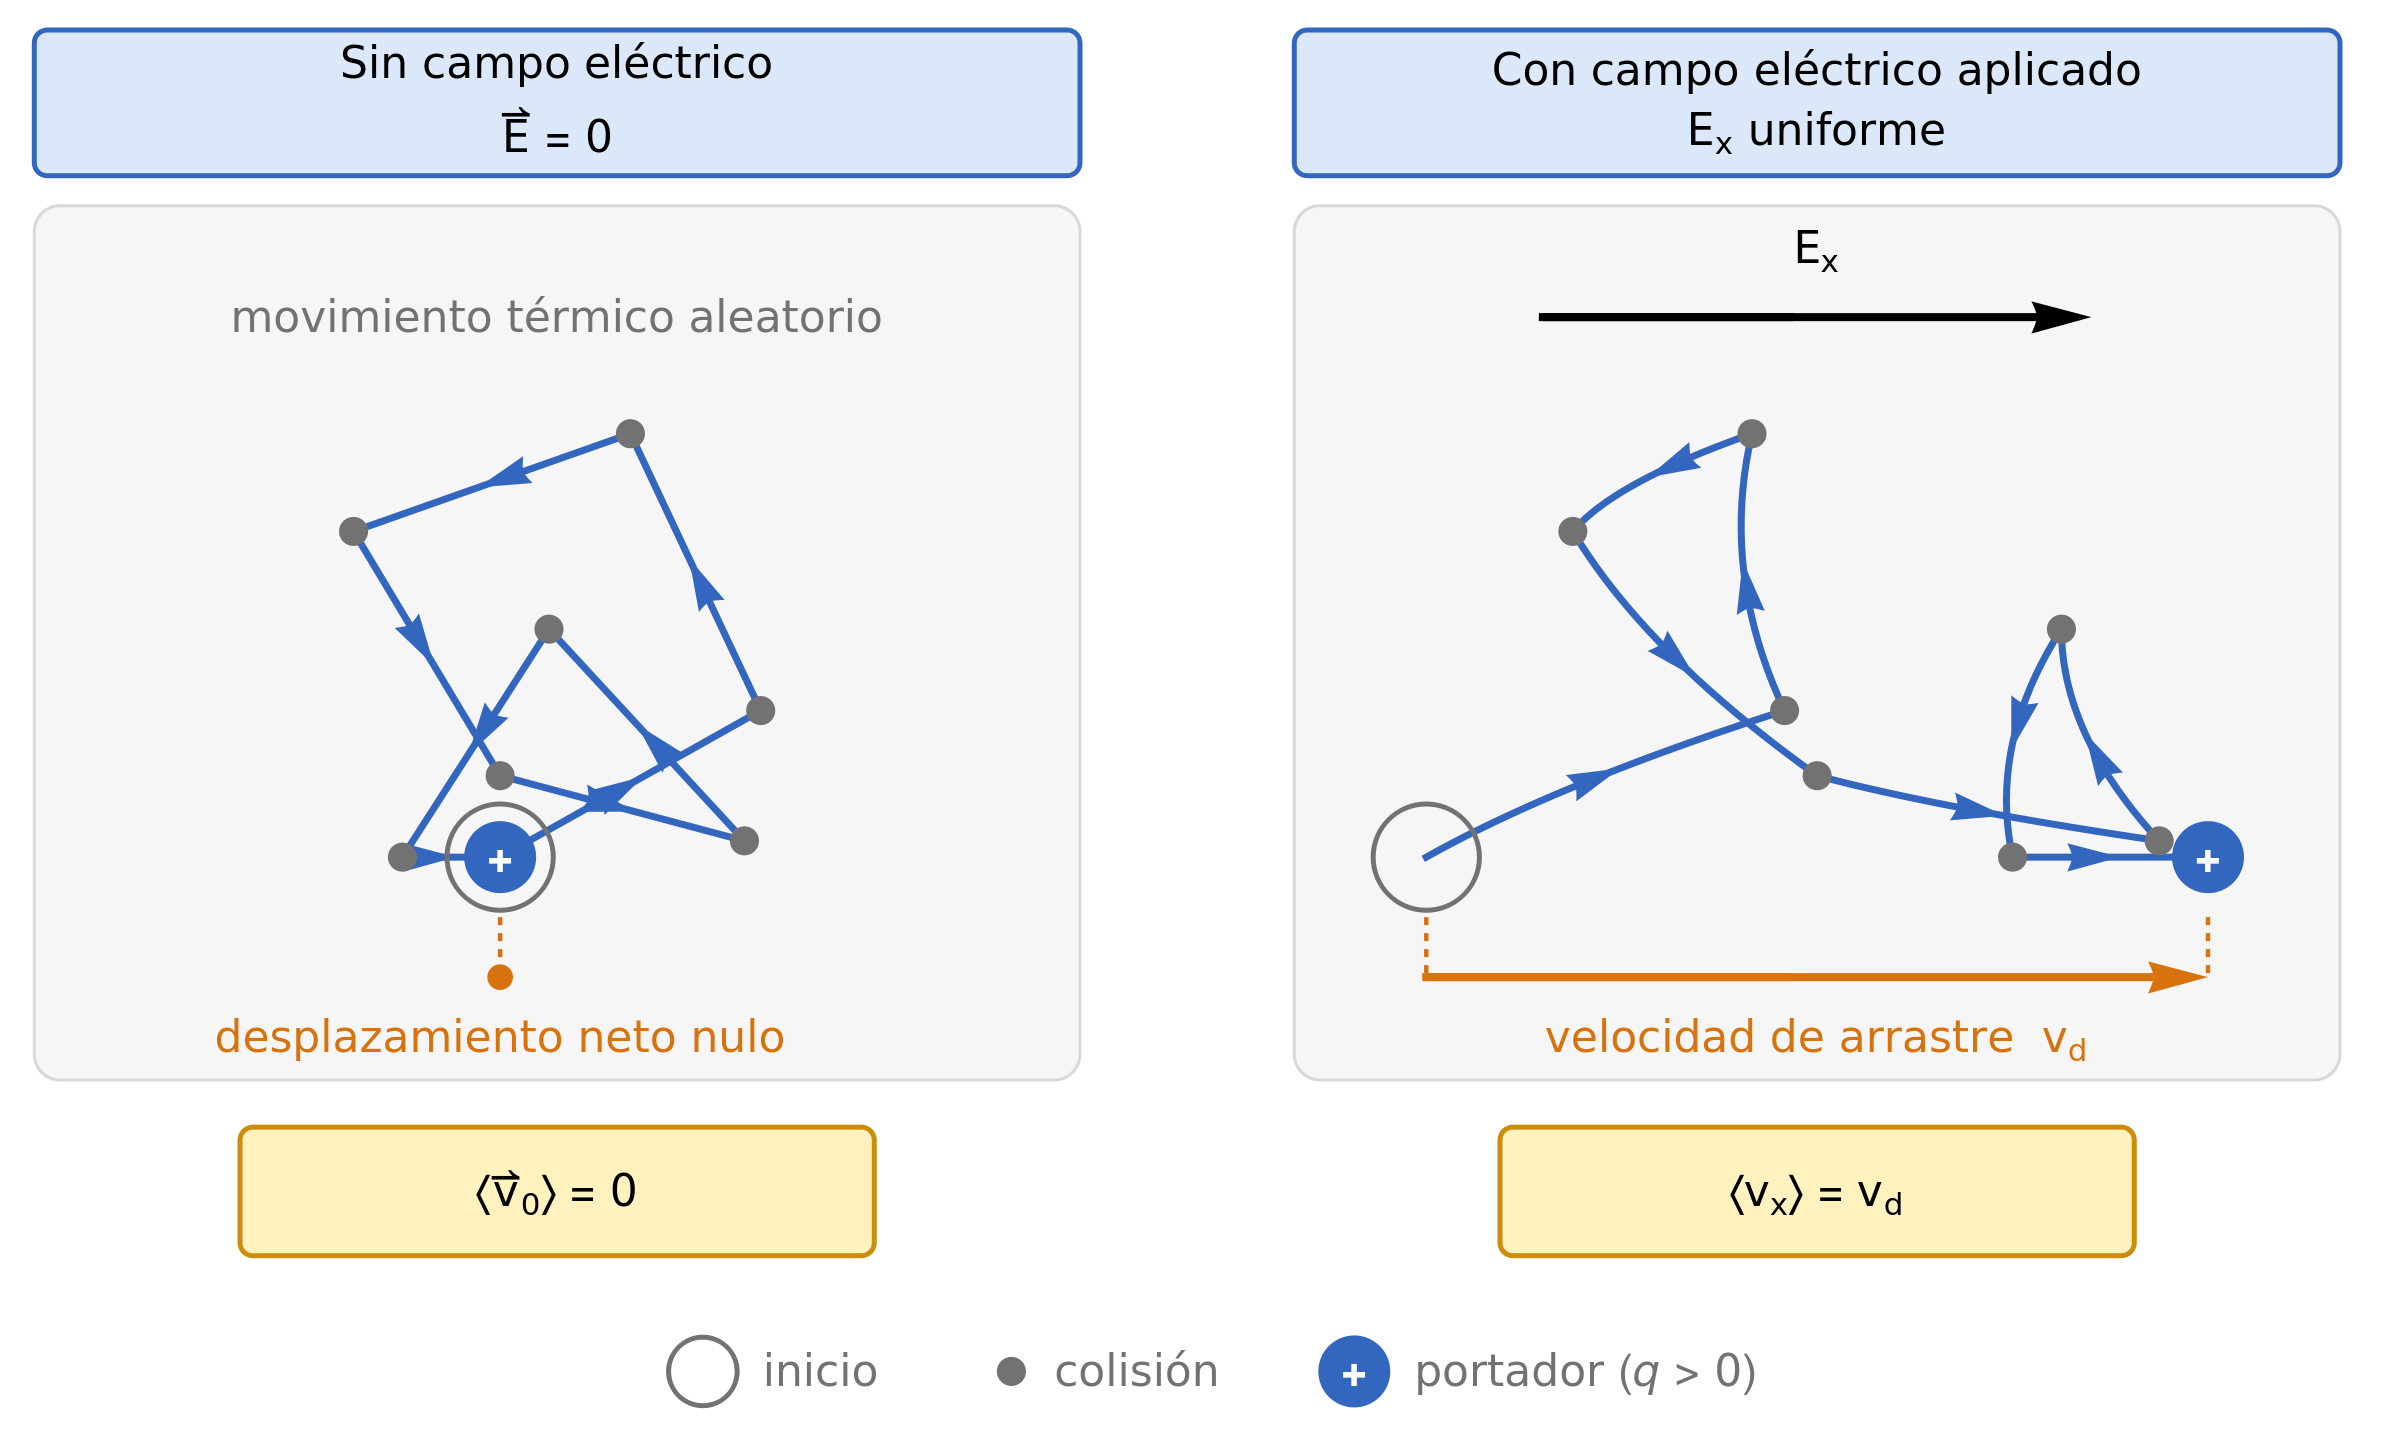
\includegraphics[width=0.5\textwidth]{imagenes/Tema3/T3_1.png}
    \caption{Trayectoria aleatoria de un portador de carga en la red cristalina: (a) En ausencia de campo eléctrico ($E = 0$), con velocidad media nula; (b) En presencia de un campo eléctrico ($E > 0$), produciéndose un desplazamiento neto en la dirección de la fuerza eléctrica (velocidad de arrastre $v_d$).}
    \label{fig:velocidad_arrastre}
\end{figure}

\newpage
%============================================
%==== SUBSECCIÓN: VELOCIDAD Y CORRIENTE =====
%============================================
\subsection{Velocidad y corriente}

Se define la \textbf{movilidad} ($\mu_n$ para electrones y $\mu_p$ para huecos) como el factor de proporcionalidad entre la velocidad de arrastre y el campo eléctrico aplicado. Sus unidades en el Sistema Internacional y en física de semiconductores son $\si{\cm^2\per\volt\per\second}$:

\begin{itemize}
    \item \textbf{Electrones ($e^-$):} Con carga $q = -e$, masa efectiva $m_n^*$ y tiempo de relajación $\tau_n$:
    \[
    \vec{v}_{dn} = -\mu_n \vec{E} \quad \implies \quad \mu_n = \frac{e \tau_n}{m_n^*}
    \]
    \item \textbf{Huecos ($h^+$):} Con carga $q = +e$, masa efectiva $m_p^*$ y tiempo de relajación $\tau_p$:
    \[
    \vec{v}_{dp} = \mu_p \vec{E} \quad \implies \quad \mu_p = \frac{e \tau_p}{m_p^*}
    \]
\end{itemize}

\begin{concepto}[Carácter tensorial de la movilidad]
En la descripción rigurosa de cristales no isotrópicos o con superficies isoenergéticas no esféricas, la movilidad relaciona dos vectores de forma orientacional y se representa mediante un tensor de segundo rango $\boldsymbol{\mu}$ ($\vec{v}_d = \boldsymbol{\mu} \vec{E}$). Sin embargo, bajo la aproximación de bandas parabólicas e isotrópicas (superficies isoenergéticas esféricas), el tensor se reduce a un escalar diagonal con componentes idénticas.
\end{concepto}

La densidad de corriente eléctrica asociada al flujo ordenado de portadores de densidad $n$ (o $p$) a velocidad $\vec{v}_d$ es:
\[
\vec{J} = q \, n \, \vec{v}_d
\]

Sustituyendo las expresiones de la velocidad de arrastre para electrones y huecos:
\begin{align*}
\vec{J}_{an} &= (-e) \, n \, (-\mu_n \vec{E}) = e \, n \, \mu_n \vec{E} = \sigma_n \vec{E} \\
\vec{J}_{ap} &= (+e) \, p \, (\mu_p \vec{E}) = e \, p \, \mu_p \vec{E} = \sigma_p \vec{E}
\end{align*}
donde se definen las \textbf{conductividades} parciales de electrones ($\sigma_n$) y huecos ($\sigma_p$), expresadas en $(\Omega \cdot \si{\cm})^{-1}$ o $\si{\S\per\cm}$:
\[
\sigma_n = e \, n \, \mu_n \qquad \text{y} \qquad \sigma_p = e \, p \, \mu_p
\]

\begin{concepto}[Sentido relativo de las corrientes de electrones y huecos]
A pesar de que los electrones ($q = -e$) y los huecos ($q = +e$) se desplazan en sentidos opuestos en presencia de un mismo campo eléctrico $\vec{E}$, sus contribuciones a la corriente de arrastre se suman vectorialmente en el **mismo sentido** (el del campo eléctrico $\vec{E}$). Esto se debe al signo negativo combinado de la carga del electrón con su sentido opuesto de velocidad.
\end{concepto}

La \textbf{densidad de corriente de arrastre total} ($\vec{J}_a$) resulta de la suma de ambas contribuciones:
\[
\vec{J}_a = \vec{J}_{an} + \vec{J}_{ap} = (\sigma_n + \sigma_p) \vec{E} = \sigma \vec{E}
\]
donde la \textbf{conductividad total} del semiconductor ($\sigma$) viene dada por la ley de Ohm microscópica:
\[
\sigma = e \, n \, \mu_n + e \, p \, \mu_p
\]

\newpage
\begin{ejemplo}[Cálculo de la densidad de corriente de arrastre en $\text{GaAs}$]
Considerar una muestra de Arseniuro de Galio ($\text{GaAs}$) de tipo N a $T = \SI{300}{\kelvin}$ dopada con una concentración de donadores $N_d = \SI{1e16}{\cm^{-3}}$ y $N_a = 0$. Asumiendo ionización completa y datos de movilidad $\mu_n = \SI{8500}{\cm^2\per\volt\per\second}$ y $\mu_p = \SI{400}{\cm^2\per\volt\per\second}$ ($n_i = \SI{1.8e6}{\cm^{-3}}$ a $\SI{300}{\kelvin}$):
\begin{enumerate}[label=\alph*)]
    \item Determinar la concentración de portadores mayoritarios y minoritarios en equilibrio termodinámico.
    \item Calcular la densidad de corriente de arrastre total bajo un campo eléctrico aplicado $E = \SI{10}{\volt\per\cm}$.
\end{enumerate}

\tcblower

\textbf{a) Concentraciones en equilibrio:}
Puesto que $N_d \gg n_i$, la concentración de electrones mayoritarios está determinada por el dopado:
\[
n_0 \approx N_d = \SI{1e16}{\cm^{-3}}
\]
Mediante la ley de acción de masas, la concentración de huecos minoritarios es:
\[
p_0 = \frac{n_i^2}{n_0} = \frac{(\num{1.8e6})^2}{\num{1e16}} = \SI{3.24e-4}{\cm^{-3}}
\]

\textbf{b) Densidad de corriente de arrastre $J_a$:}
La densidad de corriente de arrastre total es:
\[
J_a = e (\mu_n n_0 + \mu_p p_0) E
\]
Dado que $p_0 \ll n_0$, la contribución de los huecos minoritarios a la corriente estática de arrastre es completamente despreciable ($e \mu_p p_0 \approx 0$):
\[
J_a \approx e \mu_n N_d E
\]
Sustituyendo los valores numéricos:
\[
J_a = (\num{1.6e-19} \, \si{\coulomb}) \cdot (\SI{8500}{\cm^2\per\volt\per\second}) \cdot (\SI{1e16}{\cm^{-3}}) \cdot (\SI{10}{\volt\per\cm}) = \SI{136}{\A\per\cm^2}
\]

\textbf{Comentario:} En semiconductores extrínsecos, la corriente de arrastre estacionaria está dominada de forma casi exclusiva por los portadores mayoritarios. Sin embargo, al analizar variaciones o incrementos de corriente derivados de procesos de fotogeneración ($\Delta I$), la contribución de los portadores minoritarios fotogenerados adquiere relevancia y no puede omitirse.
\end{ejemplo}

\newpage

\subsection{Ley de Ohm: de la escala microscópica a la macroscópica}

En el laboratorio de electrotecnia y circuitos se utiliza habitualmente la expresión macroscópica de la ley de Ohm:
\[
V = I \cdot R
\]
Esta formulación no es más que la consecuencia integrada a escala macroscópica de una relación lineal entre el campo eléctrico y la densidad de corriente que opera a nivel microscópico:
\[
\vec{v}_d = \mu \vec{E} \implies \vec{J} = \sigma \vec{E}
\]

\begin{concepto}[Límite de validez de la ley de Ohm microscópica]
La relación de proporcionalidad directa $\vec{J} = \sigma \vec{E}$ solo es rigurosamente válida para \textbf{campos eléctricos bajos o moderados} ($E \lesssim \SI{1e3}{\volt\per\cm}$). A campos intensos, la velocidad de arrastre se satura y la respuesta deja de ser lineal.
\end{concepto}

Para deducir la ley macroscópica a partir de la microscópica, consideremos un bloque semiconductor prismático rectangular de sección transversal de área $A$ y longitud $L$, sometido a una diferencia de potencial $V$ entre sus extremos, por el que circula una intensidad de corriente $I$:

\begin{figure}[h!]
    \centering
    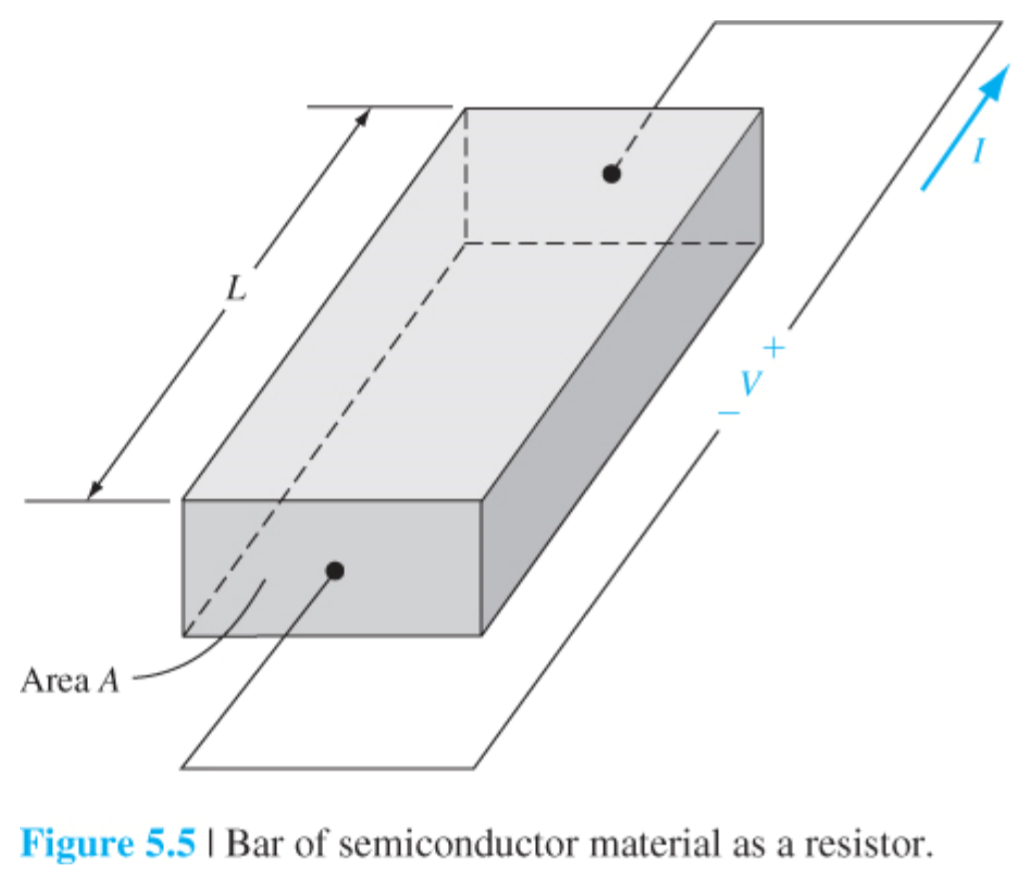
\includegraphics[width=0.6\textwidth]{imagenes/Tema3/T3_2.png}
    \caption{Geometría de una muestra semiconductora prismática sometida a una diferencia de potencial $V$, ilustrando la relación entre la densidad de corriente microscópica $\vec{J}$ y la corriente macroscópica $I$.}
    \label{fig:ohm_macroscopica}
\end{figure}

Suponiendo un campo eléctrico uniforme en el interior del cristal ($E = \frac{V}{L}$) y una densidad de corriente uniforme ($J = \frac{I}{A}$):
\[
J = \frac{I}{A} = \sigma E = \sigma \frac{V}{L}
\]

Despejando la diferencia de potencial $V$:
\[
V = \left( \frac{1}{\sigma} \frac{L}{A} \right) I = \left( \rho \frac{L}{A} \right) I = R \cdot I
\]
donde $\rho = \frac{1}{\sigma}$ es la \textbf{resistividad} del material ($\Omega \cdot \si{\cm}$) y $R = \rho \frac{L}{A}$ es la \textbf{resistencia eléctrica} macroscópica ($\Omega$).

\subsection{Efectos de campo eléctrico elevado y movilidad diferencial negativa}

A medida que el campo eléctrico aplicado aumenta por encima de $\SI{1e3}{\volt\per\cm}$, la velocidad de arrastre de los portadores deja de ser proporcional al campo. Los electrones adquieren una energía cinética media muy superior a la energía térmica de la red ($k_B T$), convirtiéndose en electrones "calientes" (\textit{hot carriers}).

\begin{figure}[h!]
    \centering
    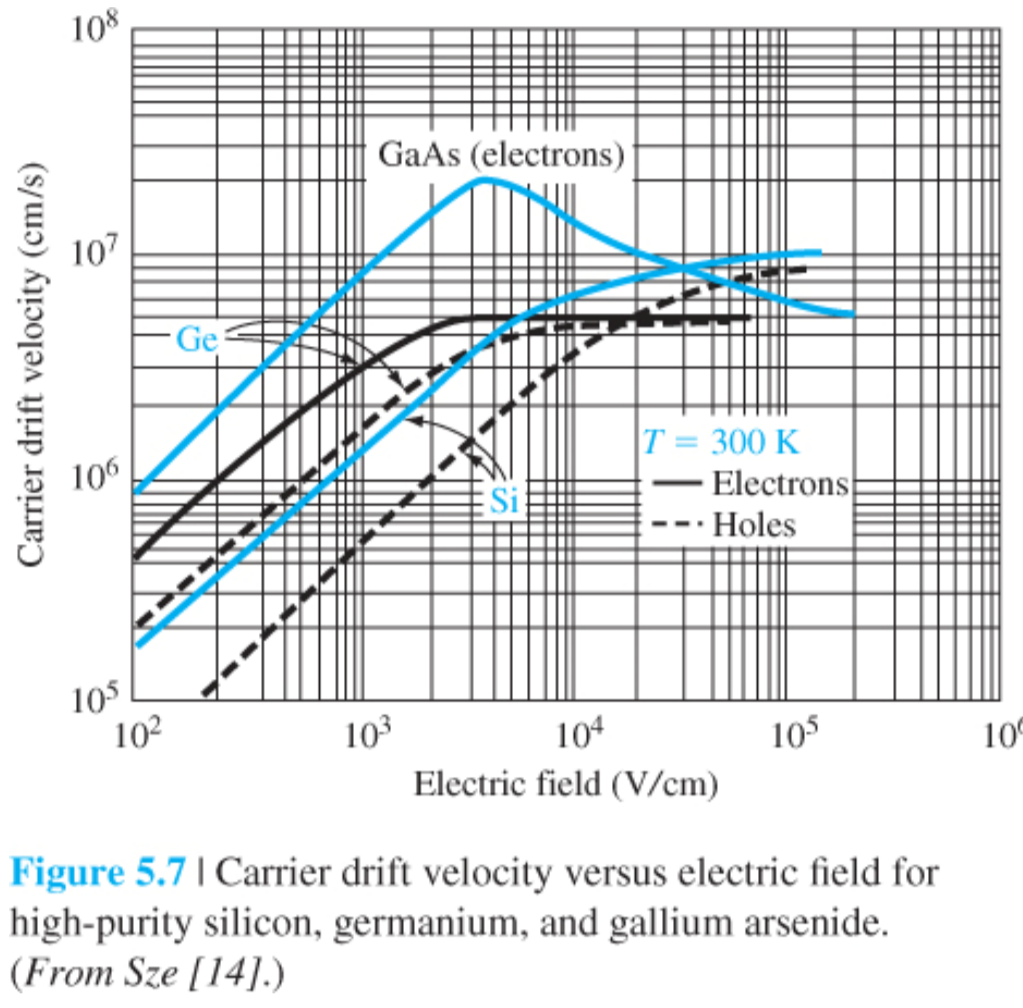
\includegraphics[width=0.65\textwidth]{imagenes/Tema3/T3_3.png}
    \caption{Curva característica de velocidad de arrastre frente a campo eléctrico ($v_d$ vs. $E$) para el Silicio y el Arseniuro de Galio, mostrando el régimen lineal de baja intensidad, la saturación de velocidad y la región de movilidad diferencial negativa.}
    \label{fig:velocidad_campo}
\end{figure}

\subsubsection{Saturación de la velocidad de arrastre}
A campos muy elevados ($E \gtrsim \SI{1e4}{\volt\per\cm}$), la velocidad de arrastre tiende asintóticamente a un valor límite constante denominado \textbf{velocidad de saturación} ($v_{\text{sat}} \approx \SI{1e7}{\cm\per\second}$ para el Si y GaAs a $\SI{300}{\kelvin}$). Esto ocurre porque la energía que el campo cede a los portadores se disipa de forma extremadamente eficiente mediante la emisión masiva de fonones ópticos de alta energía, impidiendo un mayor incremento de velocidad.

\subsubsection{Efecto de electrón transferido y movilidad diferencial negativa en $\text{GaAs}$}
En semiconductores con una estructura de bandas compleja como el Arseniuro de Galio ($\text{GaAs}$), la curva $v_d(E)$ presenta un comportamiento no monótono singular:

\begin{figure}[h!]
    \centering
    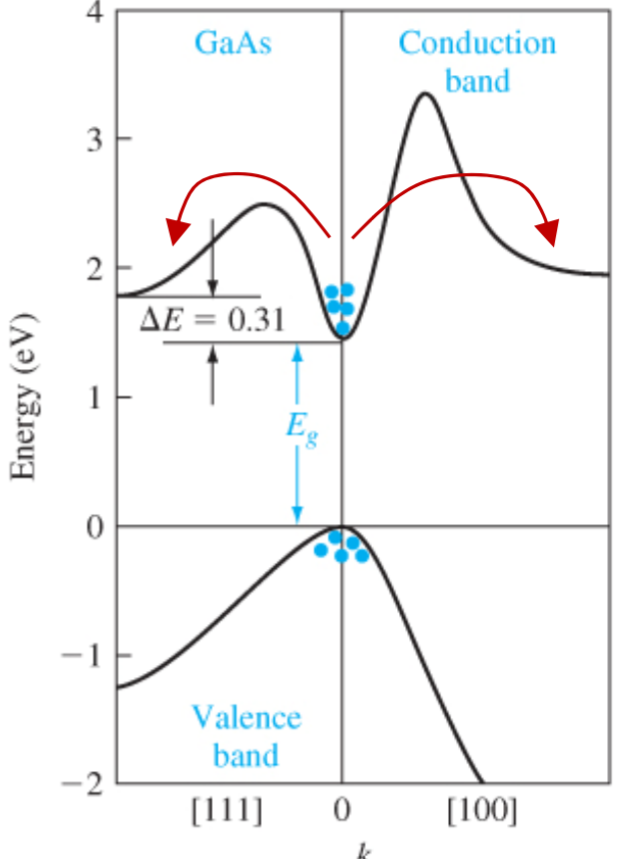
\includegraphics[width=0.7\textwidth]{imagenes/Tema3/T3_4.png}
    \caption{Estructura de la banda de conducción del $\text{GaAs}$ con el mínimo central $\Gamma$ de masa efectiva pequeña y los valles satélite $L$ de elevada masa efectiva, origen del mecanismo de transferencia electrónica (Efecto Gunn).}
    \label{fig:efecto_gunn}
\end{figure}
\begin{enumerate}
    \item \textbf{Campos bajos ($E < E_{\text{umbral}} \approx \SI{3.1}{\kilo\volt\per\cm}$):} Los electrones ocupan el mínimo central de la banda de conducción (valle $\Gamma$), caracterizado por una masa efectiva muy pequeña ($m_n^* = 0.067 m_0$) y, por ende, una movilidad muy elevada ($\mu_n \approx \SI{8500}{\cm^2\per\volt\per\second}$). La velocidad aumenta rápidamente con el campo hasta alcanzar un pico máximo $v_{\text{pico}} \approx \SI{2e7}{\cm\per\second}$.
    \item \textbf{Campos intermedios ($E > E_{\text{umbral}}$):} Los electrones ganan suficiente energía cinética para superar el salto energético ($\Delta E \approx \SI{0.31}{\eV}$) y transferirse a los valles satélite superiores (valles $L$). En estos valles, la masa efectiva es significativamente mayor ($m_n^* \approx 0.55 m_0$), lo que reduce drásticamente la movilidad ($\mu \approx \SI{100}{\cm^2\per\volt\per\second}$).
    \item \textbf{Movilidad diferencial negativa ($\mu_d < 0$):} Debido a esta transferencia de electrones hacia estados de mayor masa efectiva, al aumentar el campo eléctrico la velocidad media neta de los electrones \textbf{disminuye}:
    \[
    \mu_d = \frac{d v_d}{d E} < 0
    \]
    Esta propiedad de \textbf{resistencia diferencial negativa} es la base del funcionamiento de los \textbf{diodos Gunn}, empleados en la generación de oscilaciones de alta frecuencia en microondas.
\end{enumerate}

\subsection{Dependencia de la movilidad con la concentración de impurezas}

La movilidad de los portadores está determinada por la frecuencia de las colisiones que sufren en la red cristalina. Los dos mecanismos de dispersión principales son:
\begin{enumerate}
    \item \textbf{Dispersión por vibraciones de la red (fonones) ($\mu_L$):} Deformaciones periódicas de la red cristalina producidas por la agitación térmica.
    \item \textbf{Dispersión por impurezas ionizadas ($\mu_I$):} Interacción coulombiana atrayente o repulsiva entre los portadores en movimiento y los iones dopantes fijados a la red cristalina ($N_d^+$, $N_a^-$).
\end{enumerate}

Aplicando la \textbf{Regla de Matthiessen}, la tasa total de colisiones es la suma de las tasas parciales de cada mecanismo, lo que se traduce en la siguiente relación de movilidades:
\[
\frac{1}{\mu} = \frac{1}{\mu_L} + \frac{1}{\mu_I}
\]

\begin{figure}[h!]
    \centering
    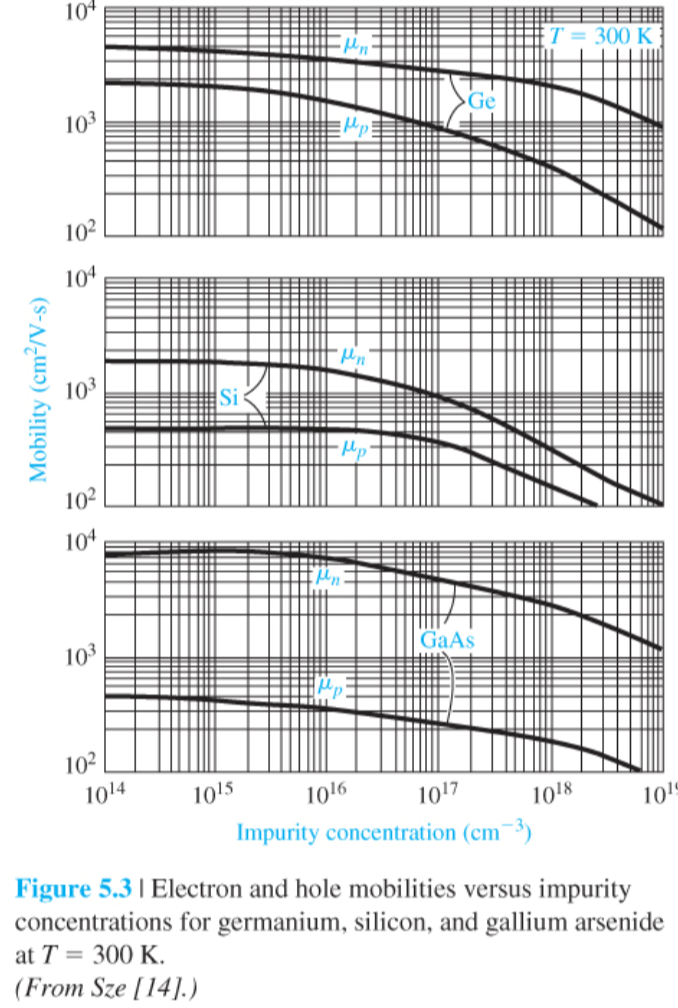
\includegraphics[width=0.7\textwidth]{imagenes/Tema3/T3_5.png}
    \caption{Variación de la movilidad de electrones y huecos en el Silicio en función de la concentración total de impurezas ionizadas ($N_d + N_a$) a $T = \SI{300}{\kelvin}$.}
    \label{fig:movilidad_impurificacion}
\end{figure}

A temperatura ambiente ($T = \SI{300}{\kelvin}$), se observan dos regiones bien diferenciadas según el nivel de dopado:
\begin{itemize}
    \item \textbf{Bajas concentraciones de impurezas ($N_d + N_a \lesssim \SI{1e15}{\cm^{-3}}$):} Las impurezas están tan distantes entre sí que la dispersión por fonones domina ampliamente ($\mu \approx \mu_L$). La movilidad alcanza su valor máximo y se mantiene sensiblemente constante.
    \item \textbf{Altas concentraciones de impurezas ($N_d + N_a \gtrsim \SI{1e15}{\cm^{-3}}$):} A medida que se incrementa el dopado, aumenta la densidad de centros con carga eléctrica que deflectan la trayectoria de los portadores. La dispersión por impurezas ionizadas ($\mu_I$) pasa a ser dominante, provocando una caída drástica de la movilidad.
\end{itemize}

\subsection{Dependencia de la movilidad con la temperatura}

La contribución de cada mecanismo de dispersión presenta una dependencia opuesta con la temperatura, lo que condiciona el comportamiento global de la movilidad $\mu(T)$:

\begin{enumerate}
    \item \textbf{Dispersión por la red ($\mu_L \propto T^{-3/2}$):} Al aumentar la temperatura, las amplitudes de vibración de los átomos de la red aumentan (mayor densidad de fonones). Esto incrementa la probabilidad de colisión y reduce el tiempo de relajación del momento, haciendo descender la movilidad.
    \item \textbf{Dispersión por impurezas ionizadas ($\mu_I \propto T^{+3/2}$):} A temperaturas elevadas, la velocidad térmica media de los portadores ($v_{\text{th}} \propto \sqrt{T}$) es más alta, por lo que las partículas transitan más rápidamente cerca de los iones dopantes. Al reducirse el tiempo de interacción, la deflexión coulombiana es menos efectiva y la movilidad $\mu_I$ aumenta con la temperatura.
\end{enumerate}

\begin{concepto}[Evolución global de $\mu(T)$ según el nivel de impurificación]
\begin{itemize}
    \item \textbf{Semiconductores poco dopados ($N_d$ bajo):} La dispersión por la red ($\mu_L$) predomina a temperatura ambiente y superior. Por tanto, la movilidad \textbf{disminuye al aumentar la temperatura} según $\mu \propto T^{-3/2}$.
    \item \textbf{Semiconductores fuertemente dopados ($N_d \sim \SI{1e19}{\cm^{-3}}$):} La dispersión por impurezas ionizadas ($\mu_I$) domina a temperaturas bajas y medias. Al superponerse la tendencia creciente de $\mu_I \propto T^{3/2}$ con la decreciente de $\mu_L \propto T^{-3/2}$, los dos efectos se compensan parcialmente, dando como resultado una movilidad mucho menor pero sensiblemente \textbf{independiente de la temperatura}.
\end{itemize}
\end{concepto}

\newpage
%============================================
%==== SUBSECCIÓN: CORRIENTE DE DIFUSIÓN =====
%============================================
\subsection{Corriente de difusión}

La \textbf{difusión} es un proceso de transporte de origen estadístico y térmico por el cual las partículas tienden a desplazarse desde zonas de alta concentración hacia zonas de menor concentración hasta homogenizar la densidad espacial.

A nivel unidimensional, la \textbf{Ley de Fick} establece que el flujo neto de partículas por unidad de área y tiempo ($F$) es proporcional y de sentido opuesto al gradiente de concentración:
\[
F = -D \frac{d N}{d x}
\]
donde $D$ es el \textbf{coeficiente de difusión} ($\si{\cm^2\per\second}$) y $N$ es la concentración local de partículas.

\subsubsection{Densidades de corriente de difusión de electrones y huecos}

Multiplicando el flujo de partículas $F$ por la carga eléctrica de cada portador ($q = -e$ para electrones y $q = +e$ para huecos), se obtienen las expresiones para las densidades de corriente de difusión:

\paragraph{a) Difusión de electrones (\texorpdfstring{$e^-$}{e-})}
Los electrones difunden en sentido contrario a su gradiente de concentración ($F_n = -D_n \frac{d n}{d x}$). Puesto que poseen carga negativa $q = -e$:
\[
J_{dn} = (-e) \cdot F_n = (-e) \cdot \left( -D_n \frac{d n}{d x} \right) \implies J_{dn} = e D_n \frac{d n}{d x}
\]
En tres dimensiones, utilizando el operador gradiente:
\[
\vec{J}_{dn} = e D_n \nabla n
\]

\paragraph{b) Difusión de huecos (\texorpdfstring{$h^+$}{h+})}
Los huecos difunden en sentido contrario a su gradiente de concentración ($F_p = -D_p \frac{d p}{d x}$). Al poseer carga positiva $q = +e$:
\[
J_{dp} = (+e) \cdot F_p = (+e) \cdot \left( -D_p \frac{d p}{d x} \right) \implies J_{dp} = -e D_p \frac{d p}{d x}
\]
En tres dimensiones:
\[
\vec{J}_{dp} = -e D_p \nabla p
\]

donde $D_n$ y $D_p$ son los \textbf{coeficientes de difusión de electrones y huecos}, respectivamente, expresados en $\si{\cm^2\per\second}$.

\begin{concepto}[Signos de las corrientes de difusión]
\begin{itemize}
    \item Si $\frac{dn}{dx} > 0$ (concentración de electrones creciente hacia la derecha), los electrones difunden hacia la izquierda. Al ser cargas negativas, producen una corriente de difusión dirigida hacia la \textbf{derecha} ($J_{dn} > 0$).
    \item Si $\frac{dp}{dx} > 0$ (concentración de huecos creciente hacia la derecha), los huecos difunden hacia la izquierda. Al ser cargas positivas, generan una corriente de difusión dirigida hacia la \textbf{izquierda} ($J_{dp} < 0$).
\end{itemize}
\end{concepto}

\begin{figure}[h!]
    \centering
    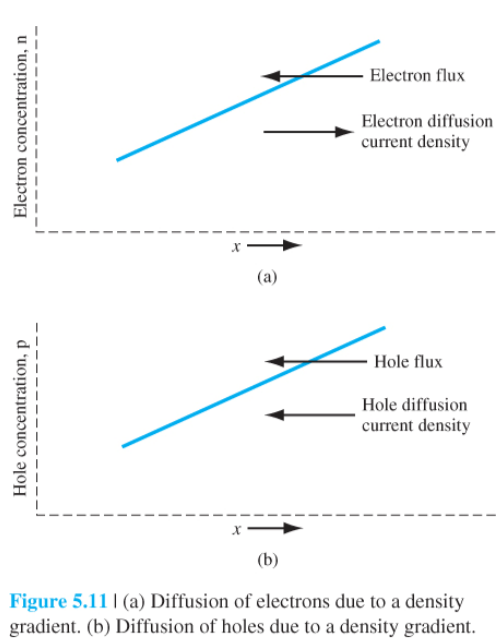
\includegraphics[width=0.4\textwidth]{imagenes/Tema3/T3_7.png}
    \caption{Difusión de a) electrones / b) huecos debido a un gradiente de densidad}
    \label{fig:difusion_signo}
\end{figure}

\newpage
\phantom{a}

\newpage
%==========================================================
%========== SUBSECCIÓN: NIVEL DE FERMI CONSTANTE===========
%==========================================================
\subsection{Nivel de Fermi constante con la posición en equilibrio}

En un semiconductor en equilibrio termodinámico (sea homogéneo o de composición e impurificación gradualmente variable), el nivel de Fermi es estrictamente constante a lo largo de toda la muestra:
\[
\frac{dE_F(x)}{dx} = 0 \implies E_F = \text{constante}
\]

\textbf{Demostración de la constancia espacial del nivel de Fermi}\\
Supongamos un semiconductor no homogéneo en el que existe un potencial eléctrico interno $V(x)$ generado por el propio gradiente de dopado (sin aplicar ningún campo externo). Debido a la presencia de este potencial, los bordes de las bandas de energía varían espacialmente según:
\[
E_C(x) = -e V(x) + E_{C0}
\]
donde $E_{C0}$ es una referencia de energía constante. El campo eléctrico interno asociado a esta curvatura de bandas es:
\[
E(x) = -\frac{dV(x)}{dx} = \frac{1}{e} \frac{dE_C(x)}{dx}
\]

Para un semiconductor de tipo N no degenerado, admitiendo que el nivel de Fermi $E_F(x)$ pudiera depender de la posición, la concentración local de electrones se expresa como:
\[
n(x) = N_C \exp\left( \frac{E_F(x) - E_C(x)}{k_B T} \right)
\]
Derivando $n(x)$ respecto a $x$:
\[
\frac{dn(x)}{dx} = N_C \exp\left( \frac{E_F(x) - E_C(x)}{k_B T} \right) \cdot \frac{1}{k_B T} \left( \frac{dE_F(x)}{dx} - \frac{dE_C(x)}{dx} \right) = \frac{n(x)}{k_B T} \left( \frac{dE_F(x)}{dx} - \frac{dE_C(x)}{dx} \right)
\]

La densidad de corriente total de electrones comprende los componentes de arrastre y difusión:
\[
J_n(x) = J_{an}(x) + J_{dn}(x) = e \mu_n n(x) E(x) + e D_n \frac{dn(x)}{dx}
\]
Sustituyendo la expresión del campo eléctrico $E(x)$, el gradiente $\frac{dn}{dx}$ y empleando la relación de Einstein ($D_n = \mu_n \frac{k_B T}{e}$):
\[
J_n(x) = e \mu_n n(x) \left( \frac{1}{e} \frac{dE_C(x)}{dx} \right) + e \left( \mu_n \frac{k_B T}{e} \right) \left[ \frac{n(x)}{k_B T} \left( \frac{dE_F(x)}{dx} - \frac{dE_C(x)}{dx} \right) \right]
\]
Simplificando los términos de la derivada del borde de la banda $E_C(x)$:
\[
J_n(x) = \mu_n n(x) \frac{dE_C(x)}{dx} + \mu_n n(x) \frac{dE_F(x)}{dx} - \mu_n n(x) \frac{dE_C(x)}{dx} = n(x) \mu_n \frac{dE_F(x)}{dx}
\]

Puesto que en equilibrio termodinámico la densidad de corriente neta de cada tipo de portador debe anularse idénticamente ($J_n = 0$), y dado que $n(x) \mu_n > 0$, se concluye necesariamente que:
\[
\frac{dE_F(x)}{dx} = 0 \implies E_F = \text{constante}
\]

\begin{figure}[h!]
    \centering
    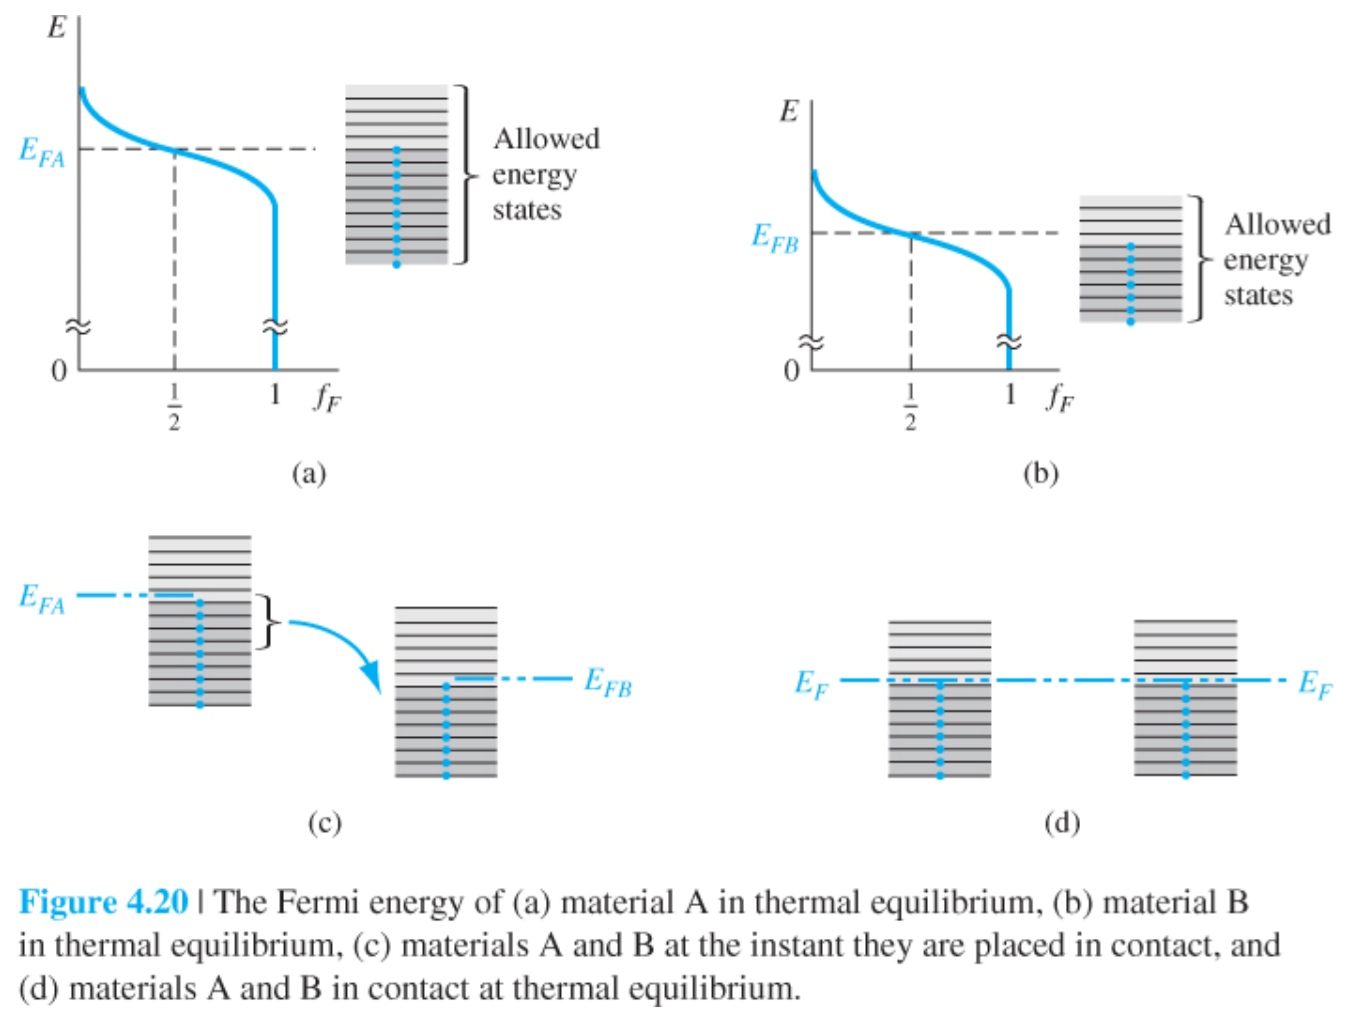
\includegraphics[width=0.7\textwidth]{imagenes/Tema3/T3_8.png}
    \caption{Diagrama de bandas de energía para un semiconductor no homogéneo en equilibrio termodinámico, donde los bordes de banda $E_C(x)$ y $E_V(x)$ se curvan espacialmente para mantener el nivel de Fermi $E_F$ estrictamente constante.}
    \label{fig:fermi_constante}
\end{figure}

\begin{concepto}[Origen físico de la curvatura de bandas]
Si unimos dos regiones semiconductoras o materiales con niveles de Fermi inicialmente distintos, se produce una difusión neta de portadores desde la zona de mayor potencial químico de electrones hacia la de menor. Esta redistribución espacial de carga crea una zona de carga de espacio con una diferencia de potencial interna $V(x)$ y un campo eléctrico $E(x)$. 

Dicho campo impulsa una corriente de arrastre que contrapone exactamente a la corriente de difusión. En el equilibrio térmico final, la alineación del nivel de Fermi ($E_F = \text{constante}$) provoca el doblamiento de los bordes de banda $E_C(x)$ y $E_V(x)$.
\end{concepto}

\newpage
%==========================================================
%========== SUBSECCIÓN: CUASINIVEL DE FERMI ===============
%==========================================================
\subsection{Cuasiniveles de Fermi}

En equilibrio termodinámico, las concentraciones de electrones ($n_0$) y huecos ($p_0$) se expresan mediante un único nivel de Fermi $E_F$:
\[
n_0 = N_C \exp\left( \frac{E_F - E_C}{k_B T} \right), \qquad p_0 = N_V \exp\left( \frac{E_V - E_F}{k_B T} \right)
\]
O bien, en función del nivel intrínseco $E_{Fi}$:
\[
n_0 = n_i \exp\left( \frac{E_F - E_{Fi}}{k_B T} \right), \qquad p_0 = n_i \exp\left( \frac{E_{Fi} - E_F}{k_B T} \right)
\]
cumpliéndose estrictamente la ley de acción de masas $n_0 \cdot p_0 = n_i^2$.

\begin{figure}[h!]
    \centering
    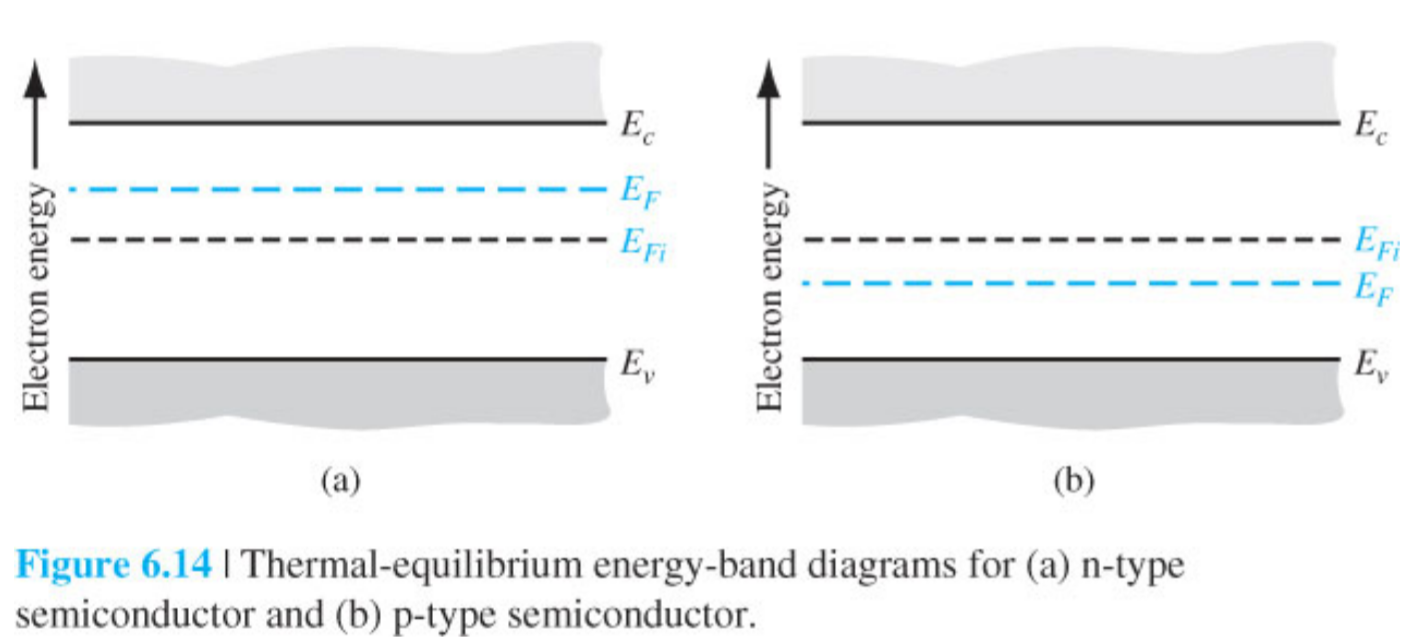
\includegraphics[width=0.65\textwidth]{imagenes/Tema3/T3_9.png}
    \caption{Posición del nivel de Fermi $E_F$ y del nivel intrínseco $E_{Fi}$ en equilibrio termodinámico para un semiconductor extrínseco.}
    \label{fig:fermi_equilibrio}
\end{figure}

Cuando el semiconductor se encuentra fuera del equilibrio termodinámico (por iluminación, inyección de corriente o campos externos), se generan concentraciones en exceso de portadores ($\Delta n, \Delta p$):
\[
n = n_0 + \Delta n, \qquad p = p_0 + \Delta p
\]
En estas condiciones, $n \cdot p \neq n_i^2$, por lo que un único nivel de Fermi deja de ser válido para describir simultáneamente ambas poblaciones.

Para formalizar estadísticamente las concentraciones fuera del equilibrio conservando las expresiones de tipo Boltzmann, se definen dos **cuasiniveles de Fermi** independientes: $E_{Fn}$ para los electrones y $E_{Fp}$ para los huecos:
\[
n = N_C \exp\left( \frac{E_{Fn} - E_C}{k_B T} \right), \qquad p = N_V \exp\left( \frac{E_V - E_{Fp}}{k_B T} \right)
\]

\begin{figure}[h!]
    \centering
    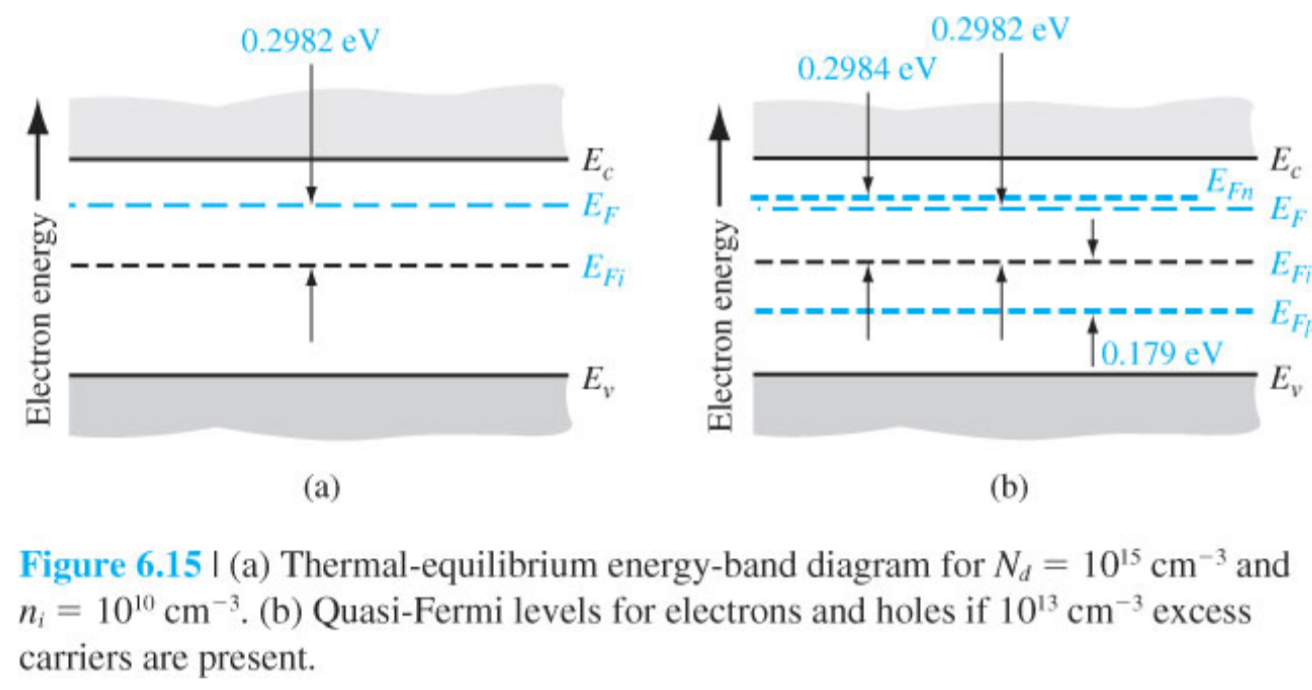
\includegraphics[width=0.7\textwidth]{imagenes/Tema3/T3_10.png}
    \caption{Separación de los cuasiniveles de Fermi $E_{Fn}$ y $E_{Fp}$ fuera del equilibrio termodinámico bajo la generación de portadores en exceso.}
    \label{fig:cuasiniveles_fermi}
\end{figure}

De forma equivalente, en función de la concentración e historia intrínseca $n_i$:
\[
n = n_i \exp\left( \frac{E_{Fn} - E_{Fi}}{k_B T} \right)
\]
\[
p = n_i \exp\left( \frac{E_{Fi} - E_{Fp}}{k_B T} \right)
\]

El producto de las concentraciones fuera del equilibrio viene dado por:
\[
n \cdot p = n_i^2 \exp\left( \frac{E_{Fn} - E_{Fp}}{k_B T} \right)
\]
La separación energética entre ambos cuasiniveles, $(E_{Fn} - E_{Fp})$, cuantifica de manera directa la desviación del sistema respecto al equilibrio termodinámico.

\newpage
\begin{ejemplo}[Cálculo de los cuasiniveles de Fermi fuera del equilibrio]
Considerar una muestra semiconductora de Silicio de tipo N a $T = \SI{300}{\kelvin}$ ($k_B T = \SI{0.0259}{\eV}$, $n_i = \SI{1.5e10}{\cm^{-3}}$) dopada con $N_d = \SI{1e15}{\cm^{-3}}$. La muestra se ilumina de forma que se genera una densidad uniforme de portadores en exceso $\Delta n = \Delta p = \SI{1e12}{\cm^{-3}}$.

\begin{enumerate}[label=\alph*)]
    \item Determinar la posición del nivel de Fermi en equilibrio ($E_F - E_{Fi}$).
    \item Obtener las posiciones de los cuasiniveles de Fermi $E_{Fn}$ y $E_{Fp}$ respecto a $E_{Fi}$ fuera del equilibrio.
\end{enumerate}

\tcblower

\textbf{a) Nivel de Fermi en equilibrio ($E_F - E_{Fi}$):}
En equilibrio, $n_0 \approx N_d = \SI{1e15}{\cm^{-3}}$ y $p_0 = \frac{n_i^2}{n_0} = \frac{(\num{1.5e10})^2}{\num{1e15}} = \SI{2.25e5}{\cm^{-3}}$.
\[
E_F - E_{Fi} = k_B T \ln\left( \frac{n_0}{n_i} \right) = (\SI{0.0259}{\eV}) \ln\left( \frac{\num{1e15}}{\num{1.5e10}} \right) \approx \SI{0.2982}{\eV}
\]

\textbf{b) Cuasiniveles de Fermi fuera del equilibrio ($E_{Fn}$ y $E_{Fp}$):}
Las concentraciones totales bajo iluminación son:
\begin{align*}
n &= n_0 + \Delta n = \SI{1e15}{\cm^{-3}} + \SI{1e12}{\cm^{-3}} = \SI{1.001e15}{\cm^{-3}} \\
p &= p_0 + \Delta p = \SI{2.25e5}{\cm^{-3}} + \SI{1e12}{\cm^{-3}} \approx \SI{1e12}{\cm^{-3}}
\end{align*}

Despejando los cuasiniveles de Fermi:
\[
E_{Fn} - E_{Fi} = k_B T \ln\left( \frac{n}{n_i} \right) = (\SI{0.0259}{\eV}) \ln\left( \frac{\num{1.001e15}}{\num{1.5e10}} \right) \approx \SI{0.2984}{\eV}
\]
\[
E_{Fi} - E_{Fp} = k_B T \ln\left( \frac{p}{n_i} \right) = (\SI{0.0259}{\eV}) \ln\left( \frac{\num{1e12}}{\num{1.5e10}} \right) \approx \SI{0.1790}{\eV}
\]

\textbf{Discusión física:}
El desplazamiento del cuasinivel de Fermi de los portadores mayoritarios ($E_{Fn}$) respecto a $E_F$ es insignificante ($\Delta E_{Fn} = \SI{0.0002}{\eV}$), ya que el exceso $\Delta n = \SI{1e12}{\cm^{-3}}$ representa una fracción mínima frente a la población de equilibrio ($n_0 = \SI{1e15}{\cm^{-3}}$).

Por el contrario, para los portadores minoritarios, la adición de $\Delta p = \SI{1e12}{\cm^{-3}}$ incrementa su concentración en casi siete órdenes de magnitud respecto a $p_0 = \SI{2.25e5}{\cm^{-3}}$. Esto desplaza notablemente el cuasinivel de Fermi de huecos $E_{Fp}$ hacia la banda de valencia, alejándose ampliamente de su posición de equilibrio.
\end{ejemplo}

\newpage

% ==========================================
% SECCIÓN 2: PROCESOS DE GENERACIÓN-RECOMBINACIÓN
% ==========================================
\section{Procesos de generación-recombinación}

Los procesos de generación y recombinación (g-r) son los mecanismos físicos que determinan la variación espacial y temporal de las concentraciones de portadores de carga en un semiconductor.

\begin{itemize}
    \item \textbf{Generación:} Consiste en la creación de un par electrón-hueco. Se produce cuando se aporta suficiente energía (de origen térmico, óptico, etc.) a un electrón de la banda de valencia para que transite a la banda de conducción.
    \item \textbf{Recombinación:} Es el proceso inverso de desexcitación. Un electrón de la banda de conducción con exceso de energía transita hacia un estado vacío en la banda de valencia, aniquilando el par electrón-hueco y cediendo su energía a la red cristalina (en forma de calor o fonones) o emitiendo un fotón.
\end{itemize}

\subsection*{Formalismo macroscópico}

A nivel macroscópico, la variación temporal de la densidad de electrones debido exclusivamente a los procesos de generación y recombinación se modela mediante la siguiente ecuación diferencial:
\[
\left. \frac{\partial n}{\partial t} \right|_{g-r} = G_{ext} - \frac{n - n_0}{\tau_n}
\]
donde:
\begin{itemize}
    \item $G_{ext}$ es la tasa de generación externa (por ejemplo, debido a iluminación, expresada en $\si{\cm^{-3}\per\second}$).
    \item $n_0$ es la concentración de electrones en equilibrio termodinámico.
    \item $n - n_0 = \delta n$ representa la concentración de portadores en exceso.
    \item $\tau_n$ es la \textbf{vida media} de los portadores en exceso (típicamente entre $\SI{1e-8}{\second}$ y $\SI{1e-3}{\second}$).
\end{itemize}

Podemos analizar la dinámica del semiconductor en dos regímenes principales:

\begin{enumerate}
    \item \textbf{Régimen estacionario:} Si la excitación externa es constante en el tiempo, se alcanza un equilibrio dinámico donde la tasa neta de variación es nula ($\frac{\partial n}{\partial t} = 0$). La concentración de portadores en exceso se estabiliza en:
    \[
    \delta n = G_{ext} \tau_n
    \]
    
    \item \textbf{Régimen transitorio (relajación):} Al cesar abruptamente la excitación externa en el instante $t = 0$ (es decir, $G_{ext} = 0$ para $t > 0$), el exceso de portadores decae exponencialmente para devolver el sistema al equilibrio térmico original:
    \[
    \delta n(t) = (G_{ext} \tau_n) \exp\left(-\frac{t}{\tau_n}\right) = \delta n(0) \exp\left(-\frac{t}{\tau_n}\right)
    \]
    donde el término $G_{ext} \tau_n$ representa la concentración inicial máxima $\delta n(0)$ justo en el momento en que cesa la excitación.
\end{enumerate}

\begin{concepto}[Tiempo de vida media total]
La vida media ($\tau$) representa el tiempo promedio que un portador permanece libre en su banda de energía antes de recombinarse. En un semiconductor real operan varios mecanismos de recombinación de forma simultánea. La vida media equivalente o efectiva se obtiene sumando las inversas de las vidas medias de cada proceso individual ($\tau_i$):
\[
\frac{1}{\tau} = \sum_i \frac{1}{\tau_i}
\]
Esto implica que el proceso de recombinación más rápido (el que posea el menor $\tau_i$) dominará la tasa de recombinación global.
\end{concepto}

\subsection{Procesos banda a banda}

Los procesos banda a banda consisten en transiciones directas de portadores entre la banda de conducción y la de valencia, y se dividen fundamentalmente en dos categorías:

\begin{itemize}
    \item \textbf{Procesos térmicos ($G_{th}, R_{th}$):} Son impulsados por la agitación térmica de la red cristalina. Son los responsables de mantener o devolver las concentraciones a los valores de equilibrio termodinámico. En condiciones de equilibrio, la tasa de generación térmica iguala a la de recombinación ($G_{th} = R_{th}$), cumpliéndose la ley de acción de masas:
    \[
    n_0 \cdot p_0 = n_i^2
    \]
    \item \textbf{Inyección (óptica o eléctrica) y perturbaciones externas ($G_L$):} Un aporte externo de energía (como la iluminación con fotones de energía $h\nu \ge E_g$) induce una generación adicional que rompe el equilibrio térmico. Esto genera un exceso de portadores en ambas bandas ($n = n_0 + \delta n$ y $p = p_0 + \delta p$). Para conservar la neutralidad de carga, generalmente $\delta n \cong \delta p$. Bajo estas condiciones, el producto de concentraciones supera al intrínseco:
    \[
    n \cdot p > n_i^2
    \]
\end{itemize}

\begin{figure}[h!]
    \centering
    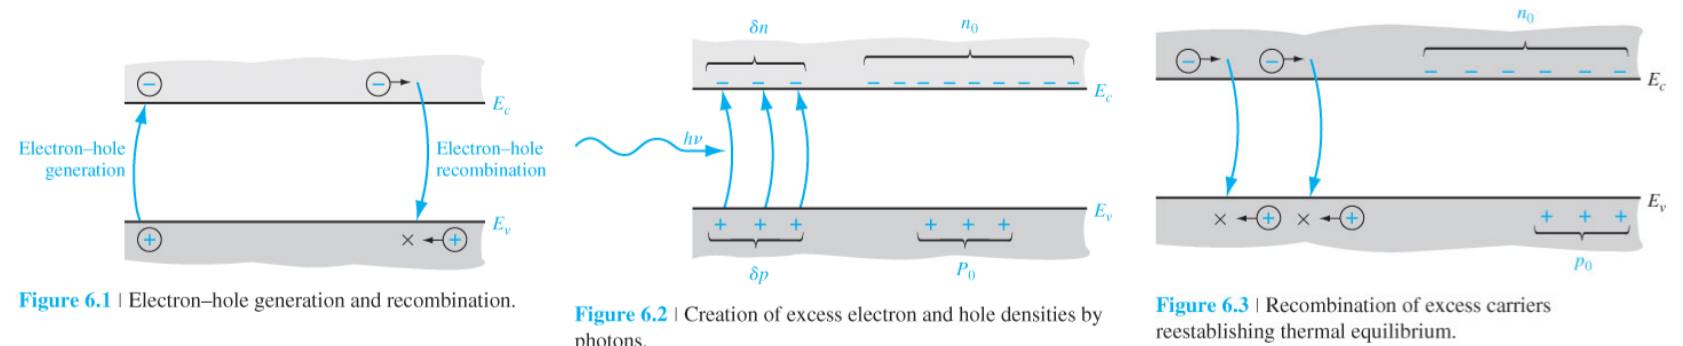
\includegraphics[width=0.7\textwidth]{imagenes/Tema3/T3_11.png}
    \caption{Esquema representativo de los procesos de generación (absorción de fotones $h\nu$) y recombinación (emisión radiativa o no radiativa) de pares electrón-hueco mediante transiciones directas banda a banda.}
    \label{fig:procesos_banda_banda}
\end{figure}

\newpage

% !TEX root = ../main.tex

\subsection{Modelo analítico de la recombinación banda a banda}

Para formular cuantitativamente la variación temporal de la concentración de portadores debido a transiciones directas entre la banda de conducción y la de valencia, se plantea el balance entre la tasa de generación y la de recombinación:
\[
\left. \frac{\partial n}{\partial t} \right|_{g-r} = \left. \frac{\partial p}{\partial t} \right|_{g-r} = G (N_V - p)(N_C - n) - c \cdot n \cdot p
\]
donde:
\begin{itemize}
    \item $G$ es la probabilidad por unidad de tiempo de generación térmica de un par.
    \item $(N_V - p)$ representa la densidad de estados ocupados (llenos de electrones) en la banda de valencia.
    \item $(N_C - n)$ representa la densidad de estados vacíos en la banda de conducción.
    \item $c$ es el \textbf{coeficiente de captura} o recombinación de electrones y huecos ($\si{\cm^3\per\second}$).
\end{itemize}

En el régimen de \textbf{débil perturbación} o semiconductor no degenerado, las concentraciones de portadores libres son muy inferiores a las densidades equivalentes de estados ($n \ll N_C$ y $p \ll N_V$). Por tanto, la densidad de estados disponibles se mantiene prácticamente constante y la ecuación se simplifica a:
\[
\left. \frac{\partial n}{\partial t} \right|_{g-r} = e - c \cdot n \cdot p
\]
donde $e = G N_V N_C$ se define como el \textbf{coeficiente de emisión} o generación térmica constante. Los coeficientes $e$ y $c$ dependen de la temperatura y de las propiedades del material, pero son independientes de $n$ y $p$.

\paragraph{Análisis en equilibrio termodinámico}
En equilibrio térmico, las concentraciones se mantienen constantes en el tiempo ($\left. \frac{\partial n}{\partial t} \right|_{g-r} = 0$), cumpliéndose la ley de acción de masas ($n_0 \cdot p_0 = n_i^2$):
\[
e - c \cdot n_0 \cdot p_0 = 0 \implies e = c \cdot n_0 \cdot p_0 = c \cdot n_i^2
\]

Sustituyendo el coeficiente de emisión $e = c \cdot n_i^2$ en la ecuación dinámica fuera del equilibrio:
\[
\left. \frac{\partial n}{\partial t} \right|_{g-r} = \left. \frac{\partial p}{\partial t} \right|_{g-r} = -c (n \cdot p - n_i^2)
\]

Igualando esta expresión con el modelo fenomenológico de tiempo de vida media ($-\frac{n - n_0}{\tau_n} = -\frac{p - p_0}{\tau_p}$):
\[
\tau_n = \tau_p = \tau = \frac{1}{c} \left( \frac{n - n_0}{n \cdot p - n_i^2} \right) = \frac{1}{c} \left( \frac{p - p_0}{n \cdot p - n_i^2} \right)
\]

\paragraph{Régimen de débil nivel de inyección}
Considerando un semiconductor extrínseco sometido a una perturbación débil de portadores en exceso ($\delta n = \delta p \ll \text{mayoritarios}$):
\[
n \cdot p - n_i^2 = (n_0 + \delta n)(p_0 + \delta p) - n_i^2 = n_0 p_0 + (n_0 + p_0)\delta p + \delta p^2 - n_i^2 \approx (n_0 + p_0)\delta p
\]

Sustituyendo esta aproximación en la fórmula del tiempo de vida media:
\[
\tau = \frac{1}{c} \frac{\delta p}{(n_0 + p_0)\delta p} = \frac{1}{c (n_0 + p_0)}
\]

Dependiendo del tipo de impurificación dominante, el tiempo de vida media del exceso de portadores toma un valor constante e independiente del nivel de inyección ($\delta n, \delta p$):
\begin{itemize}
    \item \textbf{Semiconductor tipo P ($p_0 \gg n_0$):}
    \[
    \tau = \tau_{np^+} = \frac{1}{c \cdot p_0}
    \]
    \item \textbf{Semiconductor tipo N ($n_0 \gg p_0$):}
    \[
    \tau = \tau_{pn^+} = \frac{1}{c \cdot n_0}
    \]
\end{itemize}

\newpage
%========================================================
%======= SUBSECCIÓN. PROCESOS A TRAVÉS DE CENTROS =======
%========================================================
\subsection{Procesos a través de centros de recombinación (Modelo de Shockley-Read-Hall)}

En semiconductores con gap indirecto (como el Silicio y el Germanio), las transiciones directas banda a banda son muy poco probables. La recombinación ocurre fundamentalmente a través de niveles energéticos discretos $E_T$ situados dentro de la banda prohibida, creados por defectos cristalinos o impurezas profundas (\textit{trampas} o \textit{centros recombinantes}).

\begin{figure}[h!]
    \centering
    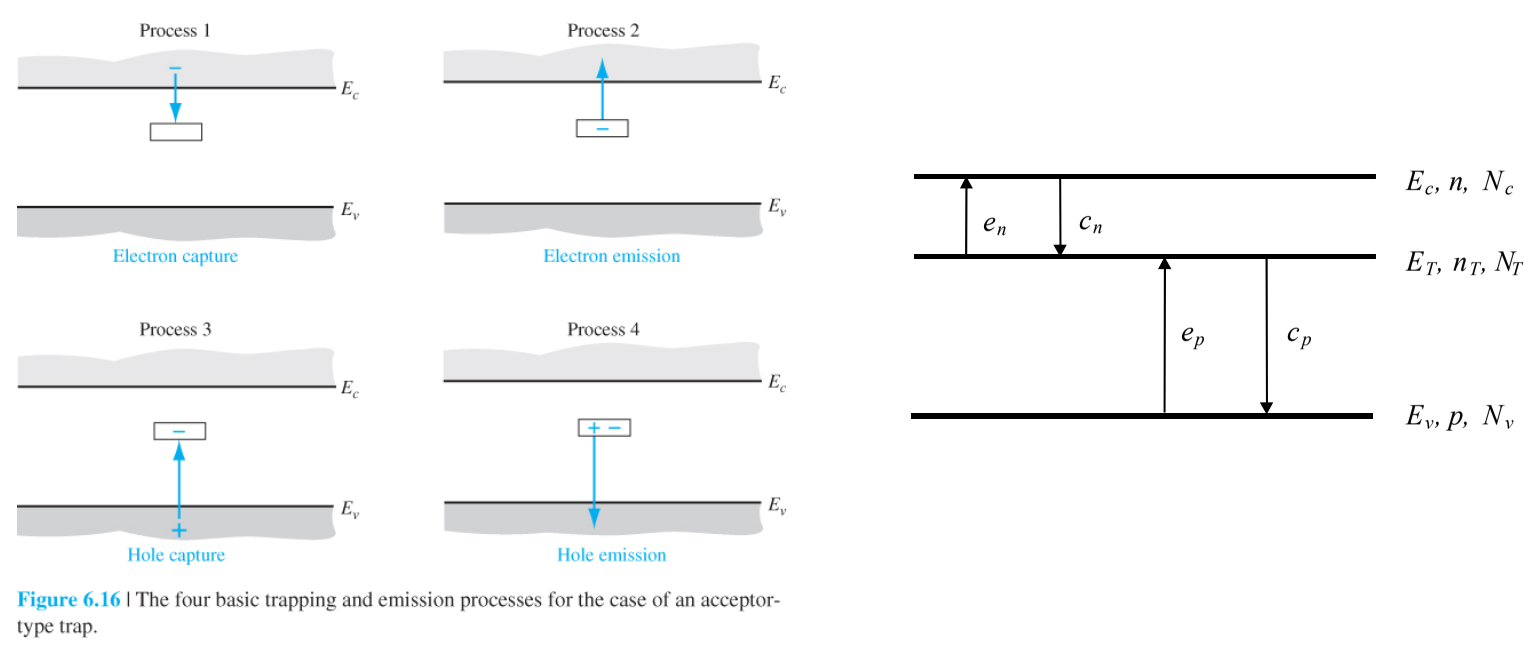
\includegraphics[width=0.75\textwidth]{imagenes/Tema3/T3_12.png}
    \caption{Los cuatro procesos elementales de trampa y emisión a través de un centro de recombinación con energía $E_T$: (1) Captura de electrón, (2) Emisión de electrón, (3) Captura de hueco, (4) Emisión de hueco.}
    \label{fig:procesos_srh}
\end{figure}

Se definen dos concentraciones energéticas de referencia ($n^1, p^1$) que representan la densidad de portadores cuando el nivel de Fermi coincide con el nivel de la trampa $E_T$:
\[
n^1 = N_C \exp\left( \frac{E_T - E_C}{k_B T} \right), \qquad p^1 = N_V \exp\left( \frac{E_V - E_T}{k_B T} \right)
\]

Bajo condiciones estacionarias ($\delta n = \delta p$), la tasa neta de recombinación por unidad de volumen derivada por Shockley, Read y Hall (teoría SRH) a través de una densidad de centros $N_T$ es:
\[
\left. \frac{\partial n}{\partial t} \right|_{g-r)_{E_T}} = \left. \frac{\partial p}{\partial t} \right|_{g-r)_{E_T}} = g(t) - \frac{(n_0 + p_0)\delta n + \delta n^2}{\frac{n^1 + n_0 + \delta n}{c_p} + \frac{p^1 + p_0 + \delta n}{c_n}} N_T
\]
donde $c_n$ y $c_p$ son las probabilidades por unidad de tiempo de captura de electrones y huecos, respectivamente.

Escribiendo la ecuación de SRH en términos del tiempo de vida media efectivo $\tau$:
\[
\left. \frac{\partial n}{\partial t} \right|_{g-r)_{E_T}} = g(t) - \frac{\delta n}{\tau} = g(t) - \frac{\delta p}{\tau}
\]
donde el tiempo de vida media $\tau$ viene dado por:
\[
\begin{array}{rl}
    \tau & = \displaystyle \frac{1}{N_T c_p} \left( \frac{n^1 + n_0 + \delta n}{n_0 + p_0 + \delta n} \right) + \frac{1}{N_T c_n} \left( \frac{p^1 + p_0 + \delta n}{n_0 + p_0 + \delta n} \right) = \\[8pt]
     & \displaystyle =  \tau_{pn^+} \left( \frac{n^1 + n_0 + \delta n}{n_0 + p_0 + \delta n} \right) + \tau_{np^+} \left( \frac{p^1 + p_0 + \delta n}{n_0 + p_0 + \delta n} \right)
\end{array}
\]

\begin{concepto}[Vida media en débil nivel de inyección]
En un semiconductor extrínseco bajo débil nivel de inyección ($\delta n \ll \text{mayoritarios}$):
\begin{itemize}
    \item \textbf{Semiconductor tipo N ($n_0 \gg p_0, n^1, p^1$):}
    \[
    \tau = \tau_{pn^+} = \frac{1}{N_T c_p}
    \]
    \item \textbf{Semiconductor tipo P ($p_0 \gg n_0, n^1, p^1$):}
    \[
    \tau = \tau_{np^+} = \frac{1}{N_T c_n}
    \]
\end{itemize}
Para diseñar dispositivos de alta velocidad de conmutación que requieran tiempos de vida media $\tau$ extremadamente cortos, se introducen intencionadamente impurezas con:
\begin{enumerate}
    \item Elevada densidad de centros ($N_T$ grande).
    \item Niveles situados cerca del centro de la banda prohibida ($E_T \approx \frac{E_g}{2}$), lo cual minimiza $n^1$ y $p^1$ y maximiza la tasa de captura.
\end{enumerate}
\end{concepto}
\newpage
%========================================================
%======= SUBSECCIÓN. PROCESOS A TRAVÉS DE CENTROS =======
%========================================================
\subsection{Recombinación superficial}

La interrupción de la periodicidad de la red en la superficie del cristal crea enlaces colgados (\textit{dangling bonds}) y defectos estructurales que actúan como una alta densidad de centros recombinantes superficiales $N_S$ con energía $E_S$.

\begin{figure}[h!]
    \centering
    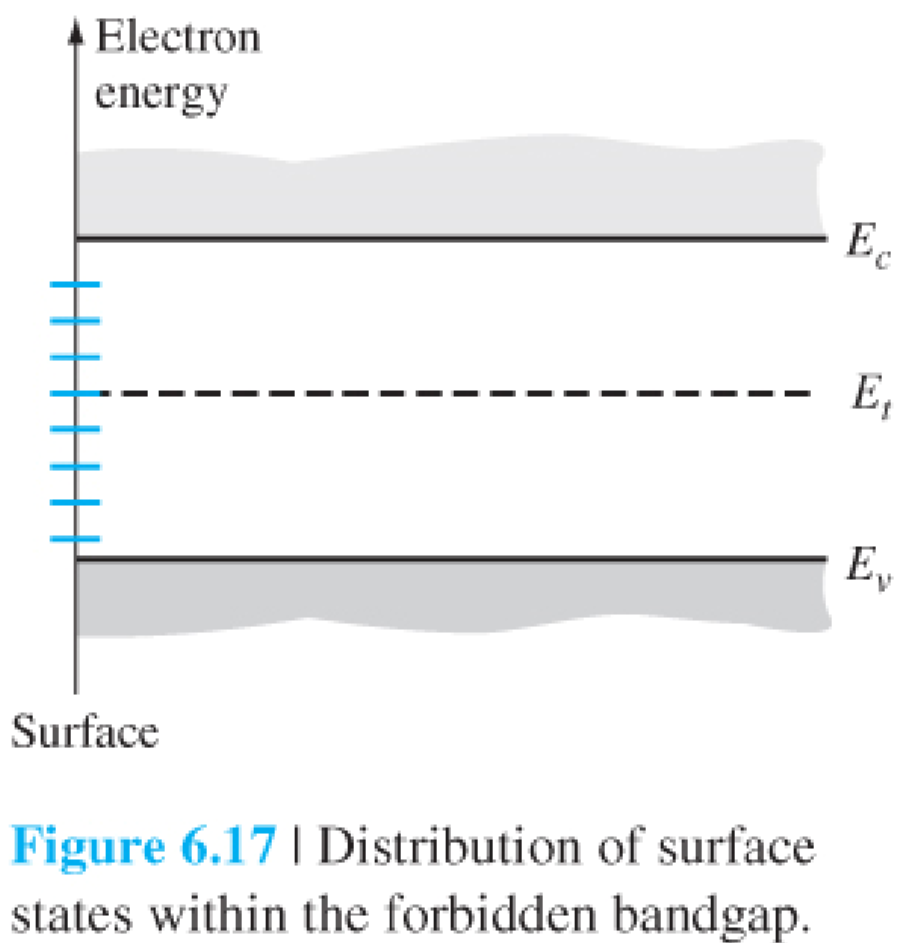
\includegraphics[width=0.5\textwidth]{imagenes/Tema3/T3_13.png}
    \caption{Distribución de estados superficiales dentro de la banda prohibida debido a la ruptura de la red cristalina en la frontera del semiconductor.}
    \label{fig:recombinacion_superficial}
\end{figure}

Aplicando la teoría SRH a la frontera del material, la tasa de recombinación superficial $R_S$ (número de portadores que se recombinan por unidad de área y tiempo, expresada en $\si{\cm^{-2}\per\second}$) es:
\[
R_S = \frac{(n_{s0} + p_{s0})\delta + \delta^2}{\frac{n_{s0} + n_s^1 + \delta}{c_{ps}} + \frac{p_{s0} + p_s^1 + \delta}{c_{ns}}} N_S
\]
donde $\delta$ es el exceso de portadores en la superficie, $n_{s0}, p_{s0}$ son las concentraciones de equilibrio superficiales, y $c_{ns}, c_{ps}$ son los coeficientes de captura superficiales.

Bajo débil nivel de inyección ($\delta \ll n_{s0}, p_{s0}$):
\[
R_S = \frac{(n_{s0} + p_{s0})\delta}{\frac{n_{s0} + n_s^1}{c_{ps}} + \frac{p_{s0} + p_s^1}{c_{ns}}} N_S
\]

\begin{concepto}[Velocidad de recombinación superficial $s$]
Se define la \textbf{velocidad de recombinación superficial} $s$ como el cociente entre la tasa de recombinación superficial $R_S$ y el exceso de portadores en la superficie $\delta$:
\[
s = \frac{R_S}{\delta} \quad \left( \si{\cm\per\second} \right)
\]
\[
s = \frac{n_{s0} + p_{s0}}{\frac{n_{s0} + n_s^1}{c_{ps}} + \frac{p_{s0} + p_s^1}{c_{ns}}} N_S
\]
En semiconductores extrínsecos bajo débil nivel de inyección:
\begin{itemize}
    \item \textbf{Tipo P ($p_{s0} \gg n_{s0}, n_s^1, p_s^1$):} $s_n = s_{np^+} = c_{ns} N_S$
    \item \textbf{Tipo N ($n_{s0} \gg p_{s0}, n_s^1, p_s^1$):} $s_p = s_{pn^+} = c_{ps} N_S$
\end{itemize}
Esta magnitud caracteriza la calidad de la pasivación de la superficie: valores altos ($s \gtrsim \SI{1e4}{\cm\per\second}$) indican superficies defectuosas con alta pérdida de portadores, mientras que valores reducidos ($s \lesssim \SI{10}{\cm\per\second}$) se obtienen mediante pasivación química u óxidos térmicos de alta calidad ($\text{SiO}_2$).
\end{concepto}
\newpage

\paragraph{Corriente de recombinación superficial y condiciones de contorno}

La recombinación de portadores en la superficie genera una \textbf{corriente de recombinación superficial} $J_{\text{rec}}$, directamente proporcional a la tasa de recombinación superficial $R_S$:
\[
J_{\text{rec}} = q R_S = q \cdot s \cdot \delta
\]
Por convenio, la corriente de recombinación superficial se define siempre apuntando hacia el exterior del volumen semiconductor (saliente por la superficie):
\begin{itemize}
    \item \textbf{Para electrones ($q = -e$):} La corriente apunta hacia el exterior con magnitud $J_{n,\text{rec}} = -e \cdot s \cdot \delta_n$.
    \item \textbf{Para huecos ($q = +e$):} La corriente apunta hacia el exterior con magnitud $J_{p,\text{rec}} = e \cdot s \cdot \delta_p$.
\end{itemize}

\begin{figure}[h!]
    \centering
    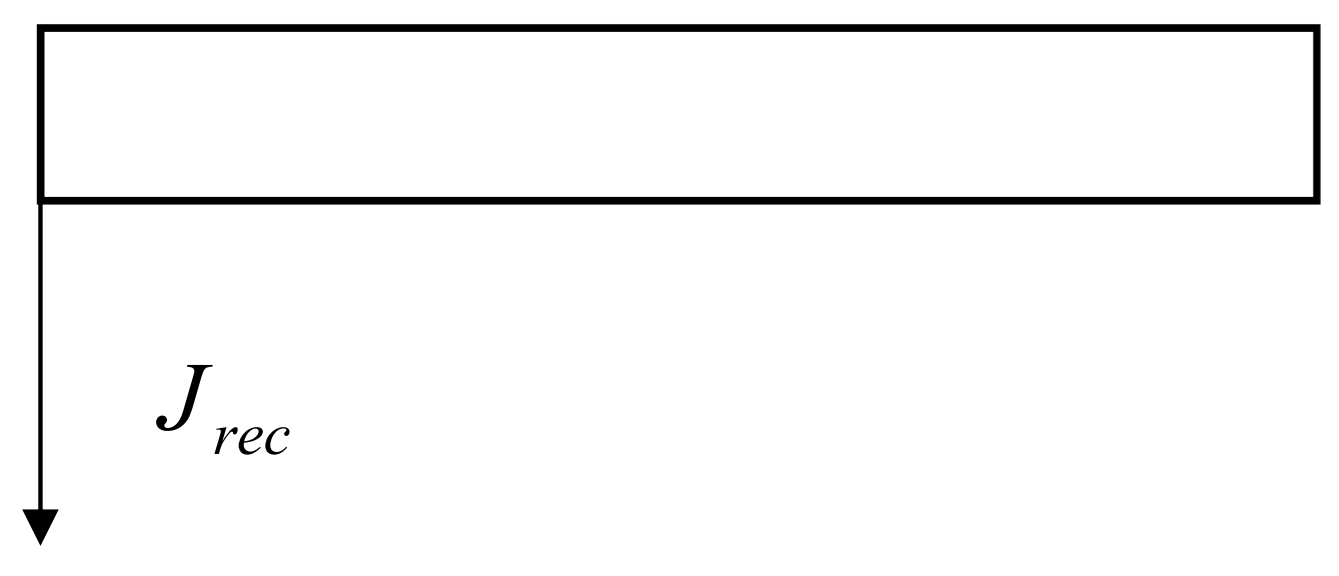
\includegraphics[width=0.4\textwidth]{imagenes/Tema3/T3_14.png}
    \caption{Representación del sentido de la corriente de recombinación superficial $J_{\text{rec}}$, saliente del volumen del semiconductor en la frontera física.}
    \label{fig:corriente_recombinacion_superficial}
\end{figure}

Esta corriente establece la \textbf{condición de contorno} necesaria para resolver la ecuación diferencial de continuidad en las fronteras del cristal. Físicamente, el flujo de portadores en exceso que llega a la superficie por difusión debe igualar exactamente a la tasa a la que se recombinan en los centros superficiales:

\begin{figure}[h!]
    \centering
    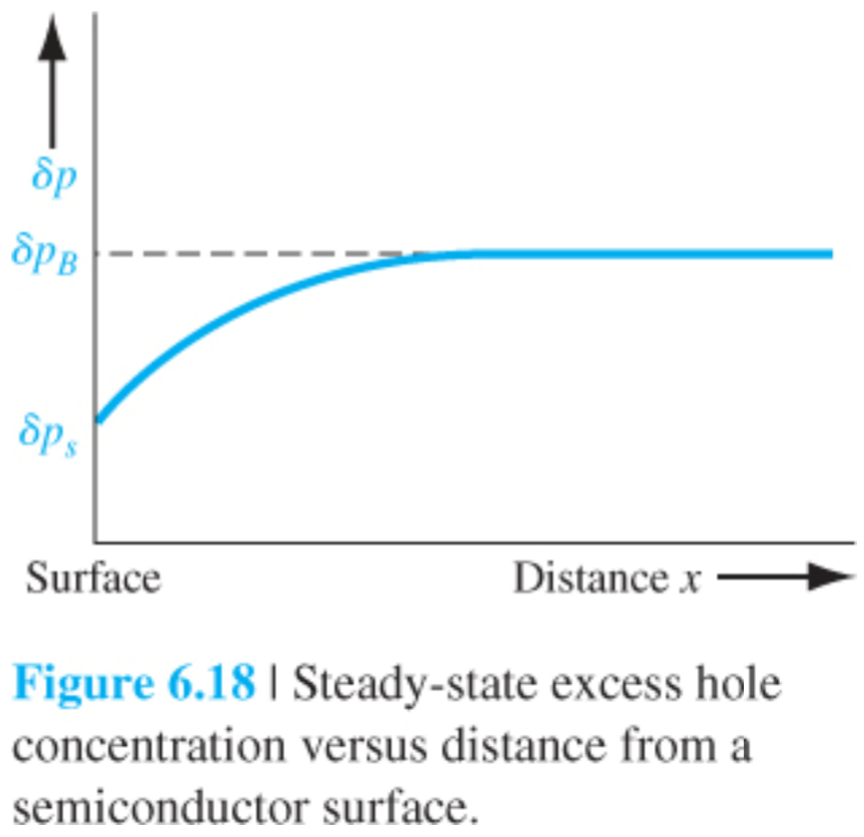
\includegraphics[width=0.65\textwidth]{imagenes/Tema3/T3_15.png}
    \caption{Balance de corrientes en la frontera: la corriente de difusión proveniente del seno del semiconductor alimenta la corriente de recombinación en la superficie.}
    \label{fig:condicion_contorno_superficial}
\end{figure}

Matemáticamente, para una frontera semiconductora en $x = 0$ (con el semiconductor extendiéndose hacia $x > 0$):
\begin{itemize}
    \item \textbf{Condición de contorno para electrones:}
    \[
    \left. D_n \frac{d(\delta n)}{dx} \right|_{x=0} = s_n \delta n(0) \implies \left. J_{dn} \right|_{x=0} = e D_n \left. \frac{d(\delta n)}{dx} \right|_{x=0} = e \cdot s_n \cdot \delta n(0)
    \]
    \item \textbf{Condición de contorno para huecos:}
    \[
    \left. D_p \frac{d(\delta p)}{dx} \right|_{x=0} = -s_p \delta p(0) \implies \left. J_{dp} \right|_{x=0} = -e D_p \left. \frac{d(\delta p)}{dx} \right|_{x=0} = e \cdot s_p \cdot \delta p(0)
    \]
\end{itemize}

\begin{figure}[h!]
    \centering
    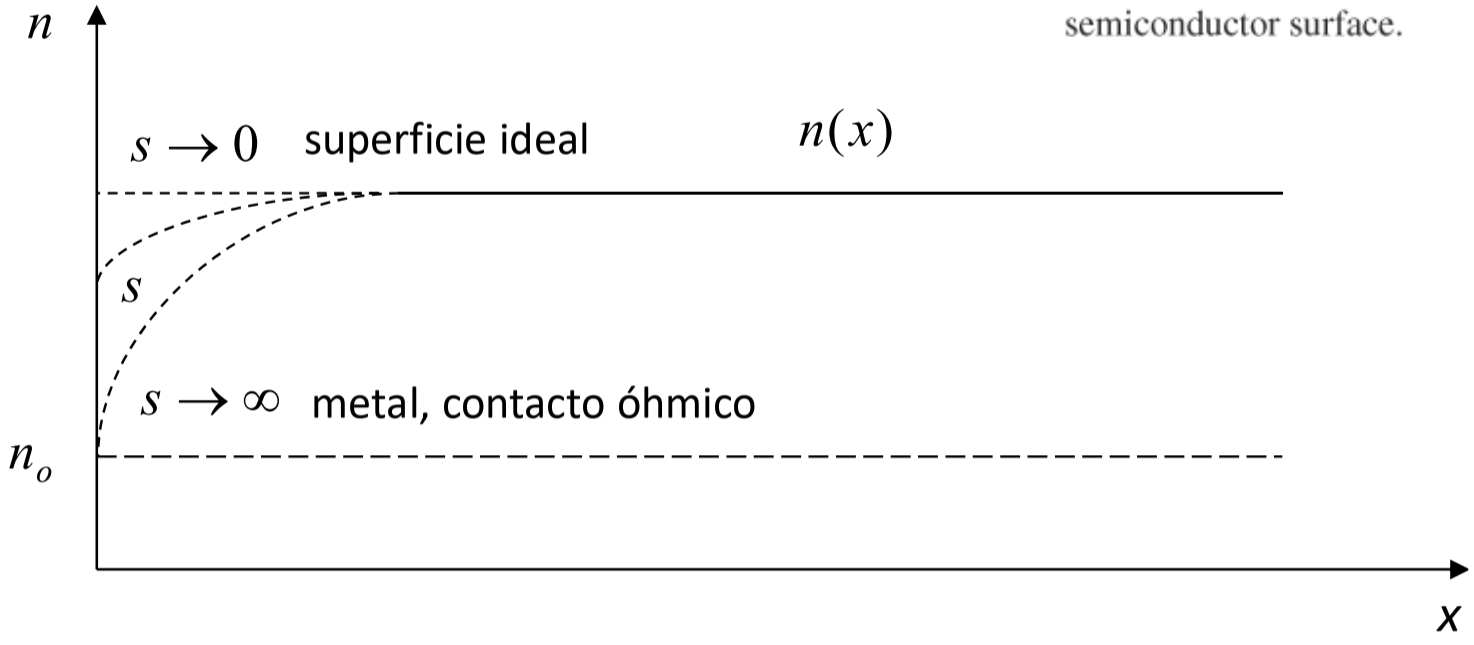
\includegraphics[width=0.65\textwidth]{imagenes/Tema3/T3_16.png}
    \caption{Gráfica}
    \label{fig:grafico_corriente_recombinacion}
\end{figure}

\newpage
\phantom{a}

\newpage
% ==========================================
% SECCIÓN 3: ECUACIÓN DE CONTINUIDAD
% ==========================================
\section{Ecuación de continuidad}

La \textbf{ecuación de continuidad} es la ecuación diferencial fundamental que gobierna la evolución espacial y temporal de las concentraciones de portadores libres ($n$ y $p$) en cualquier dispositivo semiconductor. Permite describir simultáneamente el comportamiento dinámico resultante de tres mecanismos concurrentes:
\begin{enumerate}
    \item \textbf{Flujo de corrientes de arrastre y difusión} (transporte espacial a través de los límites del elemento).
    \item \textbf{Generación de portadores} (térmica, óptica o por inyección eléctrica).
    \item \textbf{Recombinación de pares electrón-hueco}.
\end{enumerate}

\begin{figure}[h!]
    \centering
    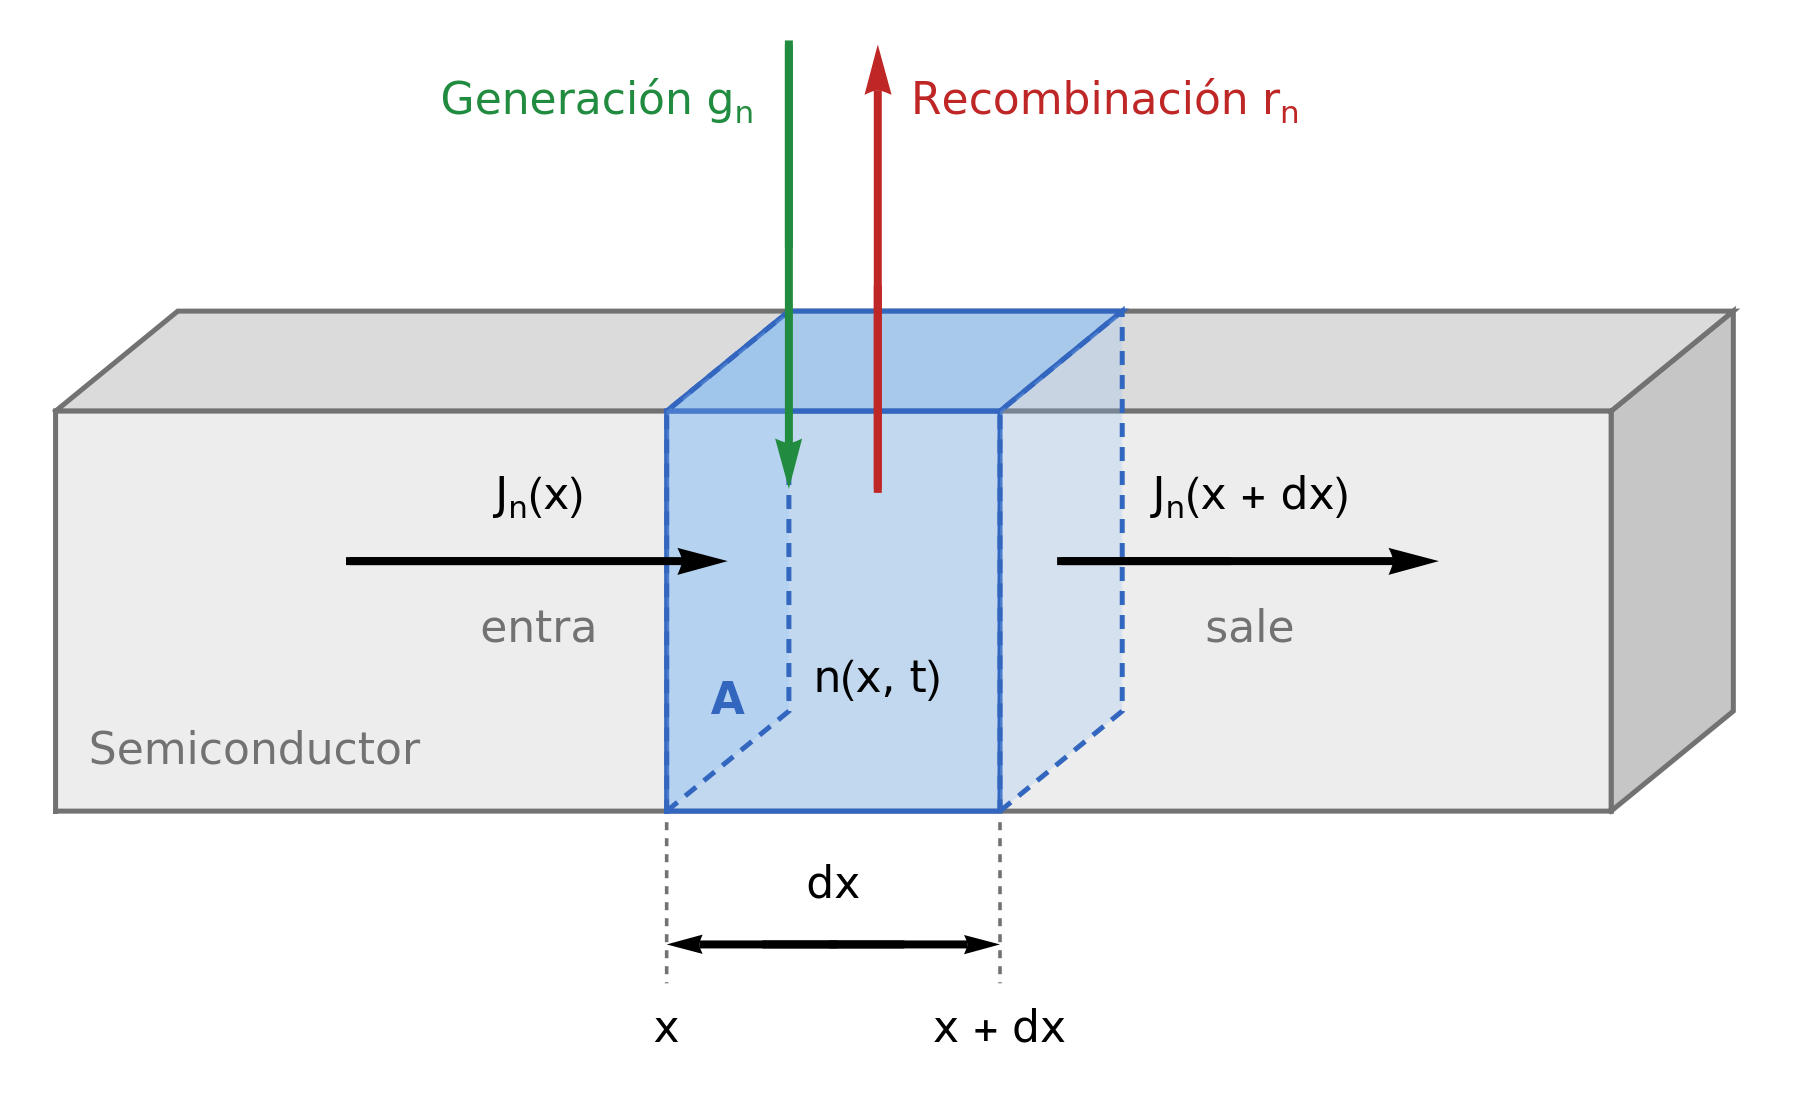
\includegraphics[width=0.7\textwidth]{imagenes/Tema3/T3_17.png}
    \caption{Elemento diferencial de volumen $A \cdot dx$ para el balance cuantitativo de acumulación, flujo entrante/saliente de corrientes y generación-recombinación de portadores.}
    \label{fig:elemento_volumen_continuidad}
\end{figure}

\subsection{Deducción del balance de carga en un elemento diferencial}

Consideremos un bloque semiconductor unidimensional con sección transversal de área $A$ y consideremos un elemento diferencial comprendido entre $x$ y $x + dx$. El volumen de esta región es $V = A \, dx$, y el número total de electrones contenidos en él viene dado por $N = n(x,t) A \, dx$.

La tasa de variación temporal del número total de electrones $N$ dentro del elemento diferencial resulta del balance estricto entre tres términos:

\begin{enumerate}
    \item \textbf{Balance de flujo por corriente eléctrica:}
    El número de electrones que entra por la cara izquierda ($x$) por unidad de tiempo es $\frac{I_n(x)}{-e} = \frac{J_n(x) A}{-e}$. 
    El número de electrones que sale por la cara derecha ($x+dx$) por unidad de tiempo es $\frac{J_n(x+dx) A}{-e}$.
    
    La contribución neta por transporte de corriente a la variación de carga interna es:
    \[
    \left. \frac{\partial N}{\partial t} \right|_{\text{corriente}} = \frac{A}{-e} \left[ J_n(x) - J_n(x+dx) \right] = \frac{A}{-e} \left( -\frac{\partial J_n}{\partial x} dx \right) = \frac{A}{e} \frac{\partial J_n}{\partial x} dx
    \]

    \item \textbf{Generación volumétrica de electrones:}
    Dada una tasa de generación total por unidad de volumen $g_n$ ($\si{\cm^{-3}\per\second}$):
    \[
    \left. \frac{\partial N}{\partial t} \right|_{\text{generación}} = g_n A \, dx
    \]

    \item \textbf{Recombinación volumétrica de electrones:}
    Dada una tasa de recombinación por unidad de volumen $r_n$ ($\si{\cm^{-3}\per\second}$):
    \[
    \left. \frac{\partial N}{\partial t} \right|_{\text{recombinación}} = -r_n A \, dx
    \]
\end{enumerate}

Sumando algebraicamente las tres contribuciones para obtener la tasa global de cambio temporal:
\[
\frac{\partial [n(x,t) A \, dx]}{\partial t} = \frac{A}{e} \frac{\partial J_n}{\partial x} dx + g_n A \, dx - r_n A \, dx
\]

Dividiendo la ecuación entre el volumen diferencial $A \, dx$, se obtiene la \textbf{ecuación de continuidad unidimensional para electrones}:
\[
\frac{\partial n}{\partial t} = \frac{1}{e} \frac{\partial J_n}{\partial x} + g_n - r_n
\]

Realizando un análisis idéntico para la población de huecos (carga $q = +e$), la corriente $I_p = J_p A$ transporta carga positiva, lo que introduce un signo negativo en el término de flujo, resultando la \textbf{ecuación de continuidad unidimensional para huecos}:
\[
\frac{\partial p}{\partial t} = -\frac{1}{e} \frac{\partial J_p}{\partial x} + g_p - r_p
\]

Generalizando a tres dimensiones mediante el operador divergencia ($\nabla \cdot \vec{J}$):

\begin{formula}[Ecuaciones generales de continuidad en 3D]
\begin{align*}
\frac{\partial n}{\partial t} &= \frac{1}{e} \nabla \cdot \vec{J}_n + g_n - r_n \\
\frac{\partial p}{\partial t} &= -\frac{1}{e} \nabla \cdot \vec{J}_p + g_p - r_p
\end{align*}
\end{formula}

\newpage

\subsubsection{Ecuación de continuidad de electrones}

La evolución temporal y espacial de la densidad de electrones en la banda de conducción $n(\vec{r},t)$ viene dada por:
\[
\frac{\partial n}{\partial t} = D_n \nabla_{\vec{r}}^2 n + \mu_n \nabla_{\vec{r}} \cdot (n \vec{E}) - \frac{n - n_0}{\tau_n} + g_L
\]
donde cada término representa un mecanismo físico diferenciado:
\begin{itemize}
    \item $D_n \nabla_{\vec{r}}^2 n$: Variación por \textbf{difusión} debido a gradientes de concentración.
    \item $\mu_n \nabla_{\vec{r}} \cdot (n \vec{E})$: Variación por \textbf{arrastre} inducido por el campo eléctrico $\vec{E}$.
    \item $-\frac{n - n_0}{\tau_n}$: Tasa neta de \textbf{generación-recombinación} de relajación hacia el equilibrio.
    \item $g_L$: Tasa de generación por \textbf{excitación externa} (óptica o eléctrica).
\end{itemize}

\subsubsection{Ecuación de continuidad de huecos}

Análogamente, para la densidad de huecos en la banda de valencia $p(\vec{r},t)$:
\[
\frac{\partial p}{\partial t} = D_p \nabla_{\vec{r}}^2 p - \mu_p \nabla_{\vec{r}} \cdot (p \vec{E}) - \frac{p - p_0}{\tau_p} + g_L
\]

\paragraph{Acoplamiento mediante la ecuación de Poisson}

Ambas ecuaciones diferenciales no son independientes, sino que se encuentran fuertemente acopladas a través del campo eléctrico $\vec{E}$ mediante la \textbf{ecuación de Poisson}:
\[
\nabla_{\vec{r}} \cdot \vec{E} = -\frac{e}{\epsilon} (n - p - N_D^+ + N_A^-)
\]
La solución analítica simultánea del sistema diferencial acoplado para determinar las distribuciones $n(\vec{r},t)$, $p(\vec{r},t)$ y $\vec{E}(\vec{r},t)$ es imposible de obtener en la inmensa mayoría de casos prácticos.

\paragraph{Formulación en términos de portadores en exceso}

Descomponiendo las concentraciones en componentes de equilibrio y perturbaciones ($n = n_0 + \delta n$, $p = p_0 + \delta p$), donde $n_0$ y $p_0$ son homogéneos e independientes de la posición y el tiempo, las ecuaciones unidimensionales de continuidad para los excesos de carga quedan expresadas como:
\begin{align}
\frac{\partial \delta n}{\partial t} &= D_n \frac{\partial^2 \delta n}{\partial x^2} + \mu_n \frac{\partial (n E)}{\partial x} - \frac{\delta n}{\tau_n} + g_L \tag{I} \\
\frac{\partial \delta p}{\partial t} &= D_p \frac{\partial^2 \delta p}{\partial x^2} - \mu_p \frac{\partial (p E)}{\partial x} - \frac{\delta p}{\tau_p} + g_L \tag{II}
\end{align}

\newpage
%==================================================
%=== SUBSECCIÓN: HIPÓTESIS DE CUASI-NEUTRALIDAD ===
%==================================================
\subsection{Hipótesis de cuasi-neutralidad eléctrica y transporte ambipolar}

Al generar un exceso local de portadores bajo un campo eléctrico aplicado $\vec{E}_{\text{app}}$, electrones y huecos tienden a separarse espacialmente. Este desplazamiento induce una pequeña densidad de carga neta que genera un campo eléctrico interno $\vec{E}_{\text{int}}$ opuesto al movimiento de separación.

\begin{figure}[h!]
    \centering
    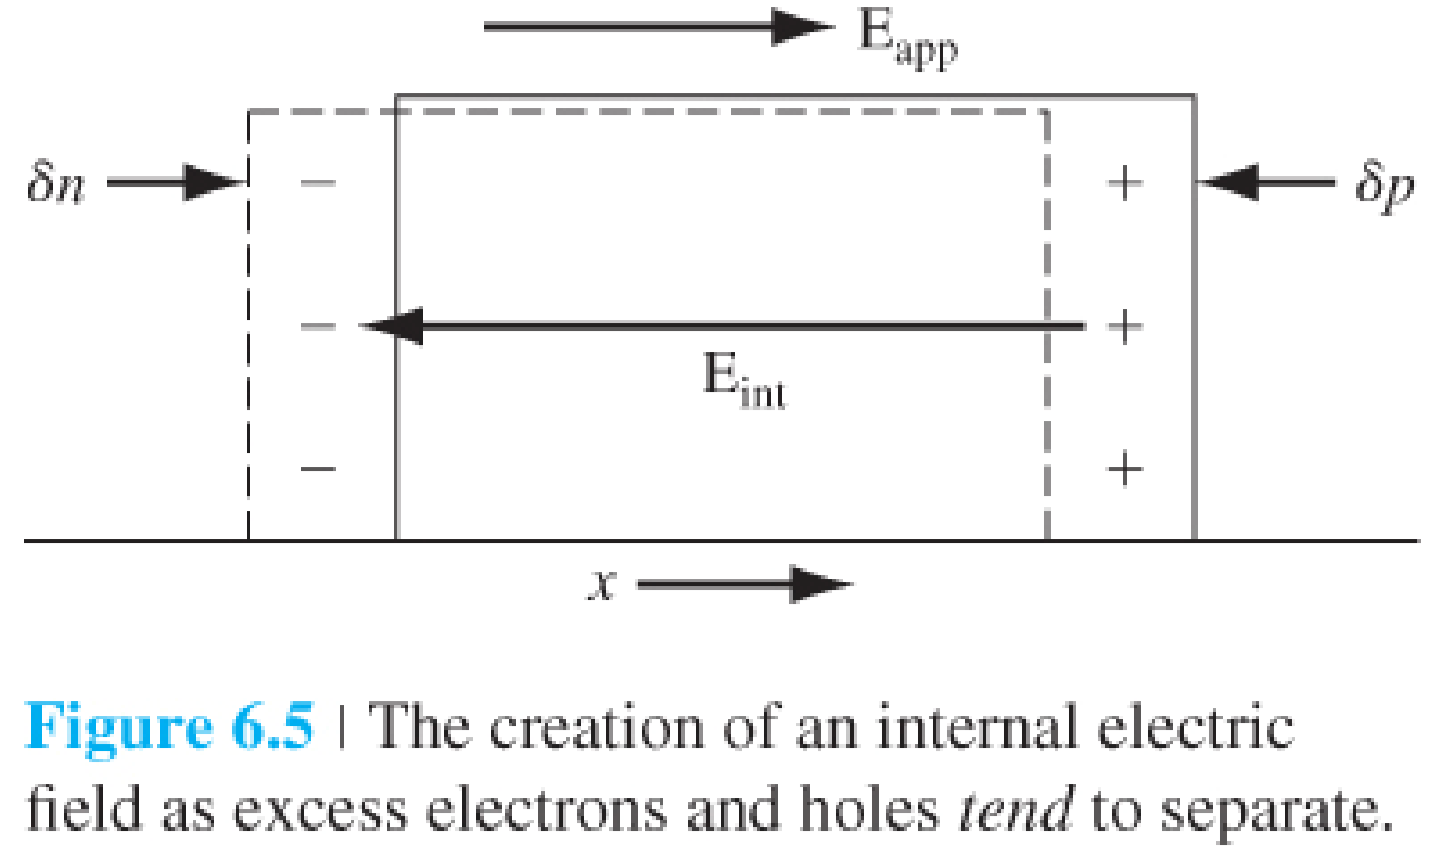
\includegraphics[width=0.65\textwidth]{imagenes/Tema3/T3_18.png}
    \caption{Creación del campo eléctrico interno $\vec{E}_{\text{int}}$ debido a la tendencia de separación espacial entre los excesos de electrones ($\delta n$) y huecos ($\delta p$).}
    \label{fig:transporte_ambipolar}
\end{figure}

El campo total en el material es $\vec{E} = \vec{E}_{\text{app}} + \vec{E}_{\text{int}}$, cuya divergencia responde a la divergencia del campo interno:
\[
\nabla_{\vec{r}} \cdot \vec{E}_{\text{int}} = -\frac{e}{\epsilon} (\delta n - \delta p)
\]
Debido a la fuerza restauradora de $\vec{E}_{\text{int}}$, ambos tipos de portadores permanecen fuertemente acoplados y se desplazan conjuntamente por arrastre y difusión. Este comportamiento coordinado se denomina \textbf{transporte ambipolar}.

En estas condiciones se adopta la \textbf{hipótesis de cuasi-neutralidad eléctrica}, que asume que el desequilibrio local de carga es inapreciable frente a la población total de portadores:
\[
\delta n = n - n_0 \approx p - p_0 = \delta p
\]

\subsubsection{Ecuación ambipolar de difusión}

Combinando algebraicamente las ecuaciones diferenciales ($\mu_p p \cdot \text{(I)} + \mu_n n \cdot \text{(II)}$), se elimina la divergencia del campo eléctrico y se obtiene la \textbf{ecuación ambipolar de difusión}:
\[
\frac{\partial \delta n}{\partial t} + \mu^* \vec{E} \cdot \nabla_{\vec{r}} \delta n - D^* \nabla_{\vec{r}}^2 \delta n + \frac{\delta n}{\tau^*} - g_L = 0
\]
donde las magnitudes efectivas ambipolares se definen como:
\begin{itemize}
    \item \textbf{Movilidad ambipolar ($\mu^*$):}
    \[
    \mu^* = \frac{\mu_n \mu_p n_0 - \mu_n \mu_p p_0}{\mu_p p + \mu_n n}
    \]
    \item \textbf{Coeficiente de difusión ambipolar ($D^*$):}
    \[
    D^* = \frac{D_n \mu_p p + \mu_n D_p n}{\mu_p p + \mu_n n}
    \]
    \item \textbf{Vida media ambipolar ($\tau^*$):}
    \[
    \tau^* = \frac{\tau_n \tau_p (\mu_p p + \mu_n n)}{\mu_p p \tau_p + \mu_n n \tau_n}
    \]
\end{itemize}

\paragraph{Casos particulares}
\begin{enumerate}
    \item \textbf{Semiconductor intrínseco ($n_0 = p_0 = n_i$):} La movilidad ambipolar se anula ($\mu^* = 0$), y los parámetros $D^*$ y $\tau^*$ resultan constantes e independientes del nivel de perturbación $\delta n$.
    \item \textbf{Semiconductor extrínseco bajo débil nivel de inyección:} 
    En un semiconductor tipo N ($n_0 \gg p_0$ y $\delta n \ll n_0$):
    \[
    D^* \approx D_p, \qquad \tau^* \approx \tau_p, \qquad \mu^* \approx \mu_p
    \]
    Los parámetros de la ecuación ambipolar coinciden exactamente con los de los \textbf{portadores minoritarios}. Por tanto, la dinámica del exceso de carga queda gobernada exclusivamente por las propiedades de los minoritarios, reduciéndose la ecuación a la ecuación de continuidad lineal de minoritarios (sin el término explícito de $\vec{E}$).
\end{enumerate}

\begin{figure}[h!]
    \centering
    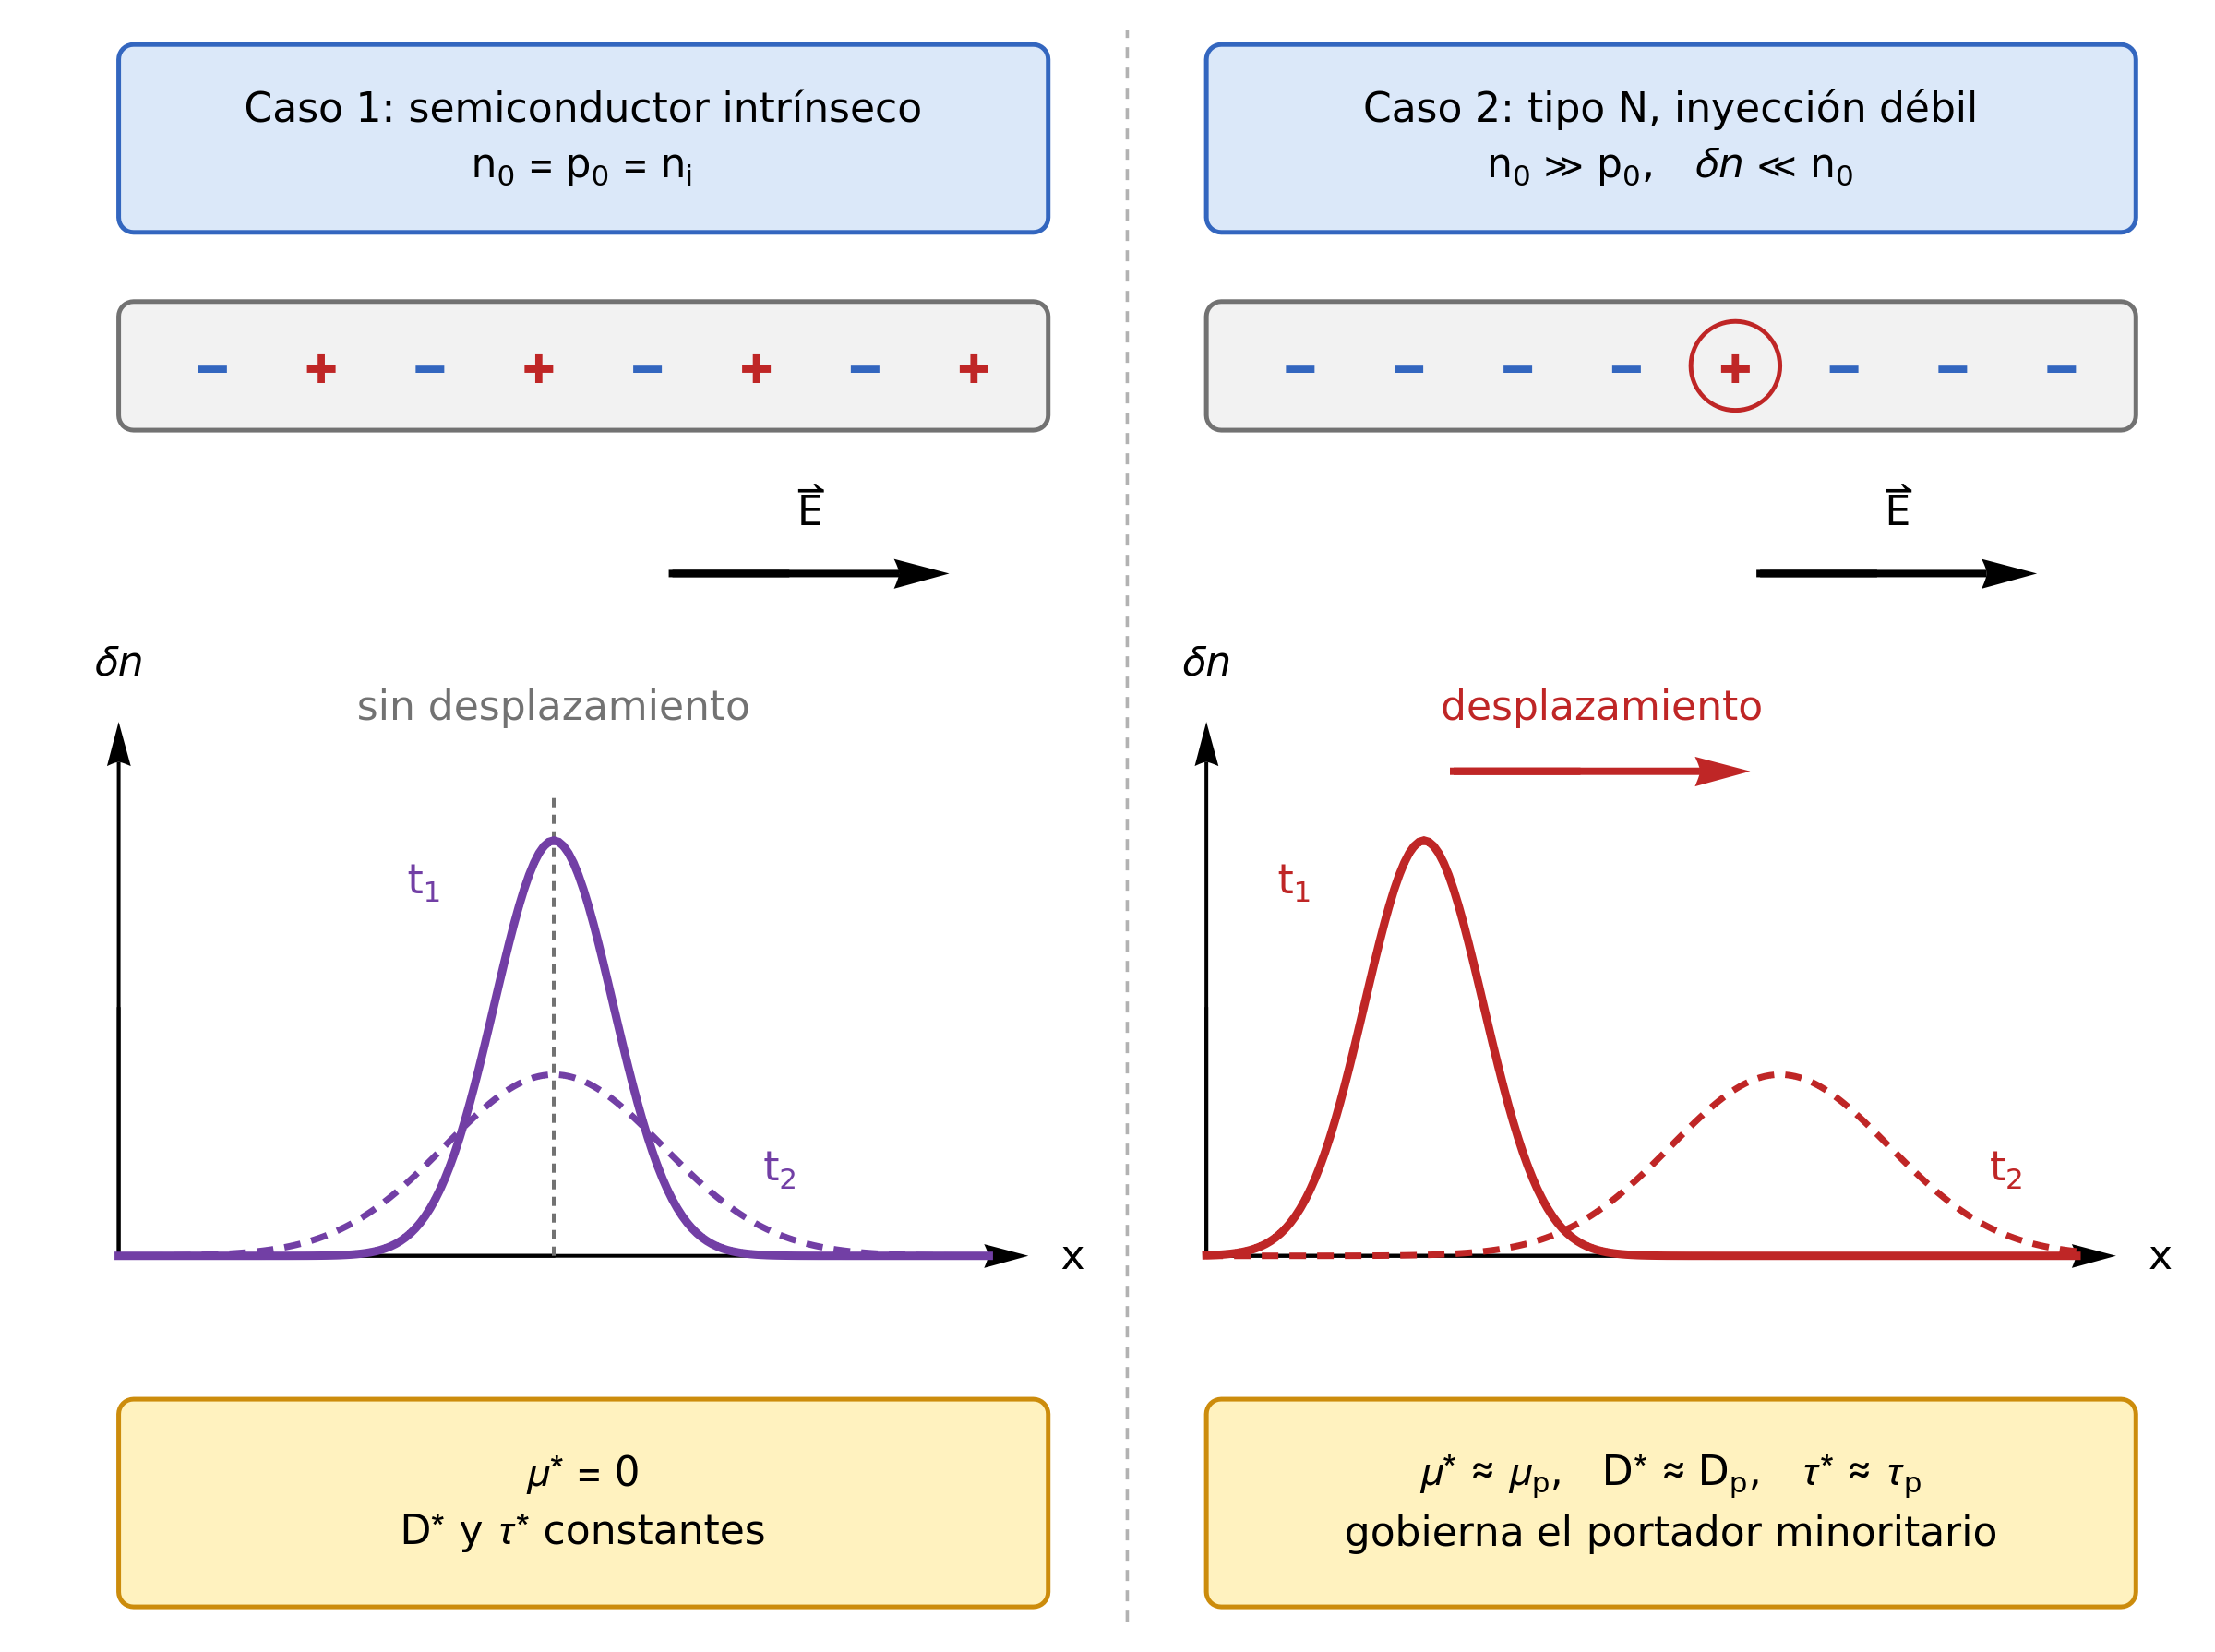
\includegraphics[width=0.75\textwidth]{imagenes/Tema3/T3_21.png}
    \caption{Casos particulares.}
    \label{fig:casos_particulares}
\end{figure}

\begin{concepto}[Metodología de cálculo para semiconductores extrínsecos]
Para resolver las distribuciones de portadores y campo eléctrico en un semiconductor extrínseco:
\begin{enumerate}
    \item \textbf{Paso 1:} Obtener la concentración en exceso resolviendo la ecuación de continuidad para portadores minoritarios despreciando el término de campo eléctrico $\vec{E} \cdot \nabla \delta n$, obteniendo $\delta n$ (o $\delta p$).
    \item \textbf{Paso 2:} Calcular las concentraciones totales mediante la hipótesis de cuasi-neutralidad:
    \[
    p = p_0 + \delta p, \qquad n = n_0 + \delta n \quad (\text{con } \delta n \approx \delta p)
    \]
    \item \textbf{Paso 3:} Determinar el campo eléctrico $\vec{E}$ despejándolo de la ecuación de continuidad de los \textbf{portadores mayoritarios}, en la cual no se desprecia el término de arrastre.
\end{enumerate}
\end{concepto}

\newpage

\begin{ejemplo}[Comportamiento temporal del exceso de portadores cuando un semiconductor vuelve al equilibrio]
Considera un semiconductor infinitamente largo, homogéneo tipo n, sin campo eléctrico aplicado ($E = 0$). A tiempo $t=0$, existe un exceso de concentración de portadores en el cristal. Suponer que $g' = 0$ para $t > 0$. Si suponemos que el exceso de concentración de portadores es mucho menor que la concentración de electrones de equilibrio térmico, la condición de débil inyección (\textit{low-injection}) es aplicable. Calcular el exceso de concentración de portadores en función del tiempo $t$.
\tcblower
Para un semiconductor tipo n, la dinámica del exceso de carga está determinada por la ecuación de continuidad/transporte ambipolar para los portadores minoritarios (huecos):
\[
D_p \frac{\partial^2 (\delta p)}{\partial x^2} - \mu_p E \frac{\partial (\delta p)}{\partial x} + g' - \frac{\delta p}{\tau_{p0}} = \frac{\partial (\delta p)}{\partial t}
\]

Aplicamos las condiciones del enunciado:
\begin{enumerate}
    \item \textbf{Homogeneidad espacial:} Puesto que la perturbación inicial es uniforme en todo el espacio del semiconductor, no existen gradientes de concentración ($\frac{\partial (\delta p)}{\partial x} = 0$ y $\frac{\partial^2 (\delta p)}{\partial x^2} = 0$). El término de difusión se anula.
    \item \textbf{Sin campo eléctrico:} $E = 0$, por lo que el término de arrastre es nulo.
    \item \textbf{Sin generación externa ($t > 0$):} $g' = 0$.
\end{enumerate}

Al no haber variación espacial, sustituimos la derivada parcial temporal por una derivada total. La ecuación diferencial se reduce a una ecuación diferencial ordinaria de primer orden:
\[
\frac{d(\delta p)}{dt} = -\frac{\delta p(t)}{\tau_{p0}}
\]

Separando variables e integrando desde $t = 0$ hasta un tiempo $t > 0$:
\[
\int_{\delta p(0)}^{\delta p(t)} \frac{d(\delta p)}{\delta p} = -\int_{0}^{t} \frac{dt'}{\tau_{p0}} \implies \ln \left( \frac{\delta p(t)}{\delta p(0)} \right) = -\frac{t}{\tau_{p0}}
\]

Tomando exponenciales en ambos lados, obtenemos el exceso de huecos minoritarios en función del tiempo:
\[
\delta p(t) = \delta p(0) \exp\left( -\frac{t}{\tau_{p0}} \right)
\]
donde $\delta p(0)$ representa el exceso de concentración de huecos presente en la muestra en el instante inicial $t = 0$.

Bajo la condición de \textbf{débil inyección} y por la \textbf{hipótesis de cuasi-neutralidad eléctrica} ($\delta n(t) \approx \delta p(t)$), el exceso de electrones mayoritarios sigue exactamente la misma ley de relajación temporal:
\[
\delta n(t) = \delta p(t) = \delta p(0) \exp\left( -\frac{t}{\tau_{p0}} \right)
\]

\newpage

\begin{center}
    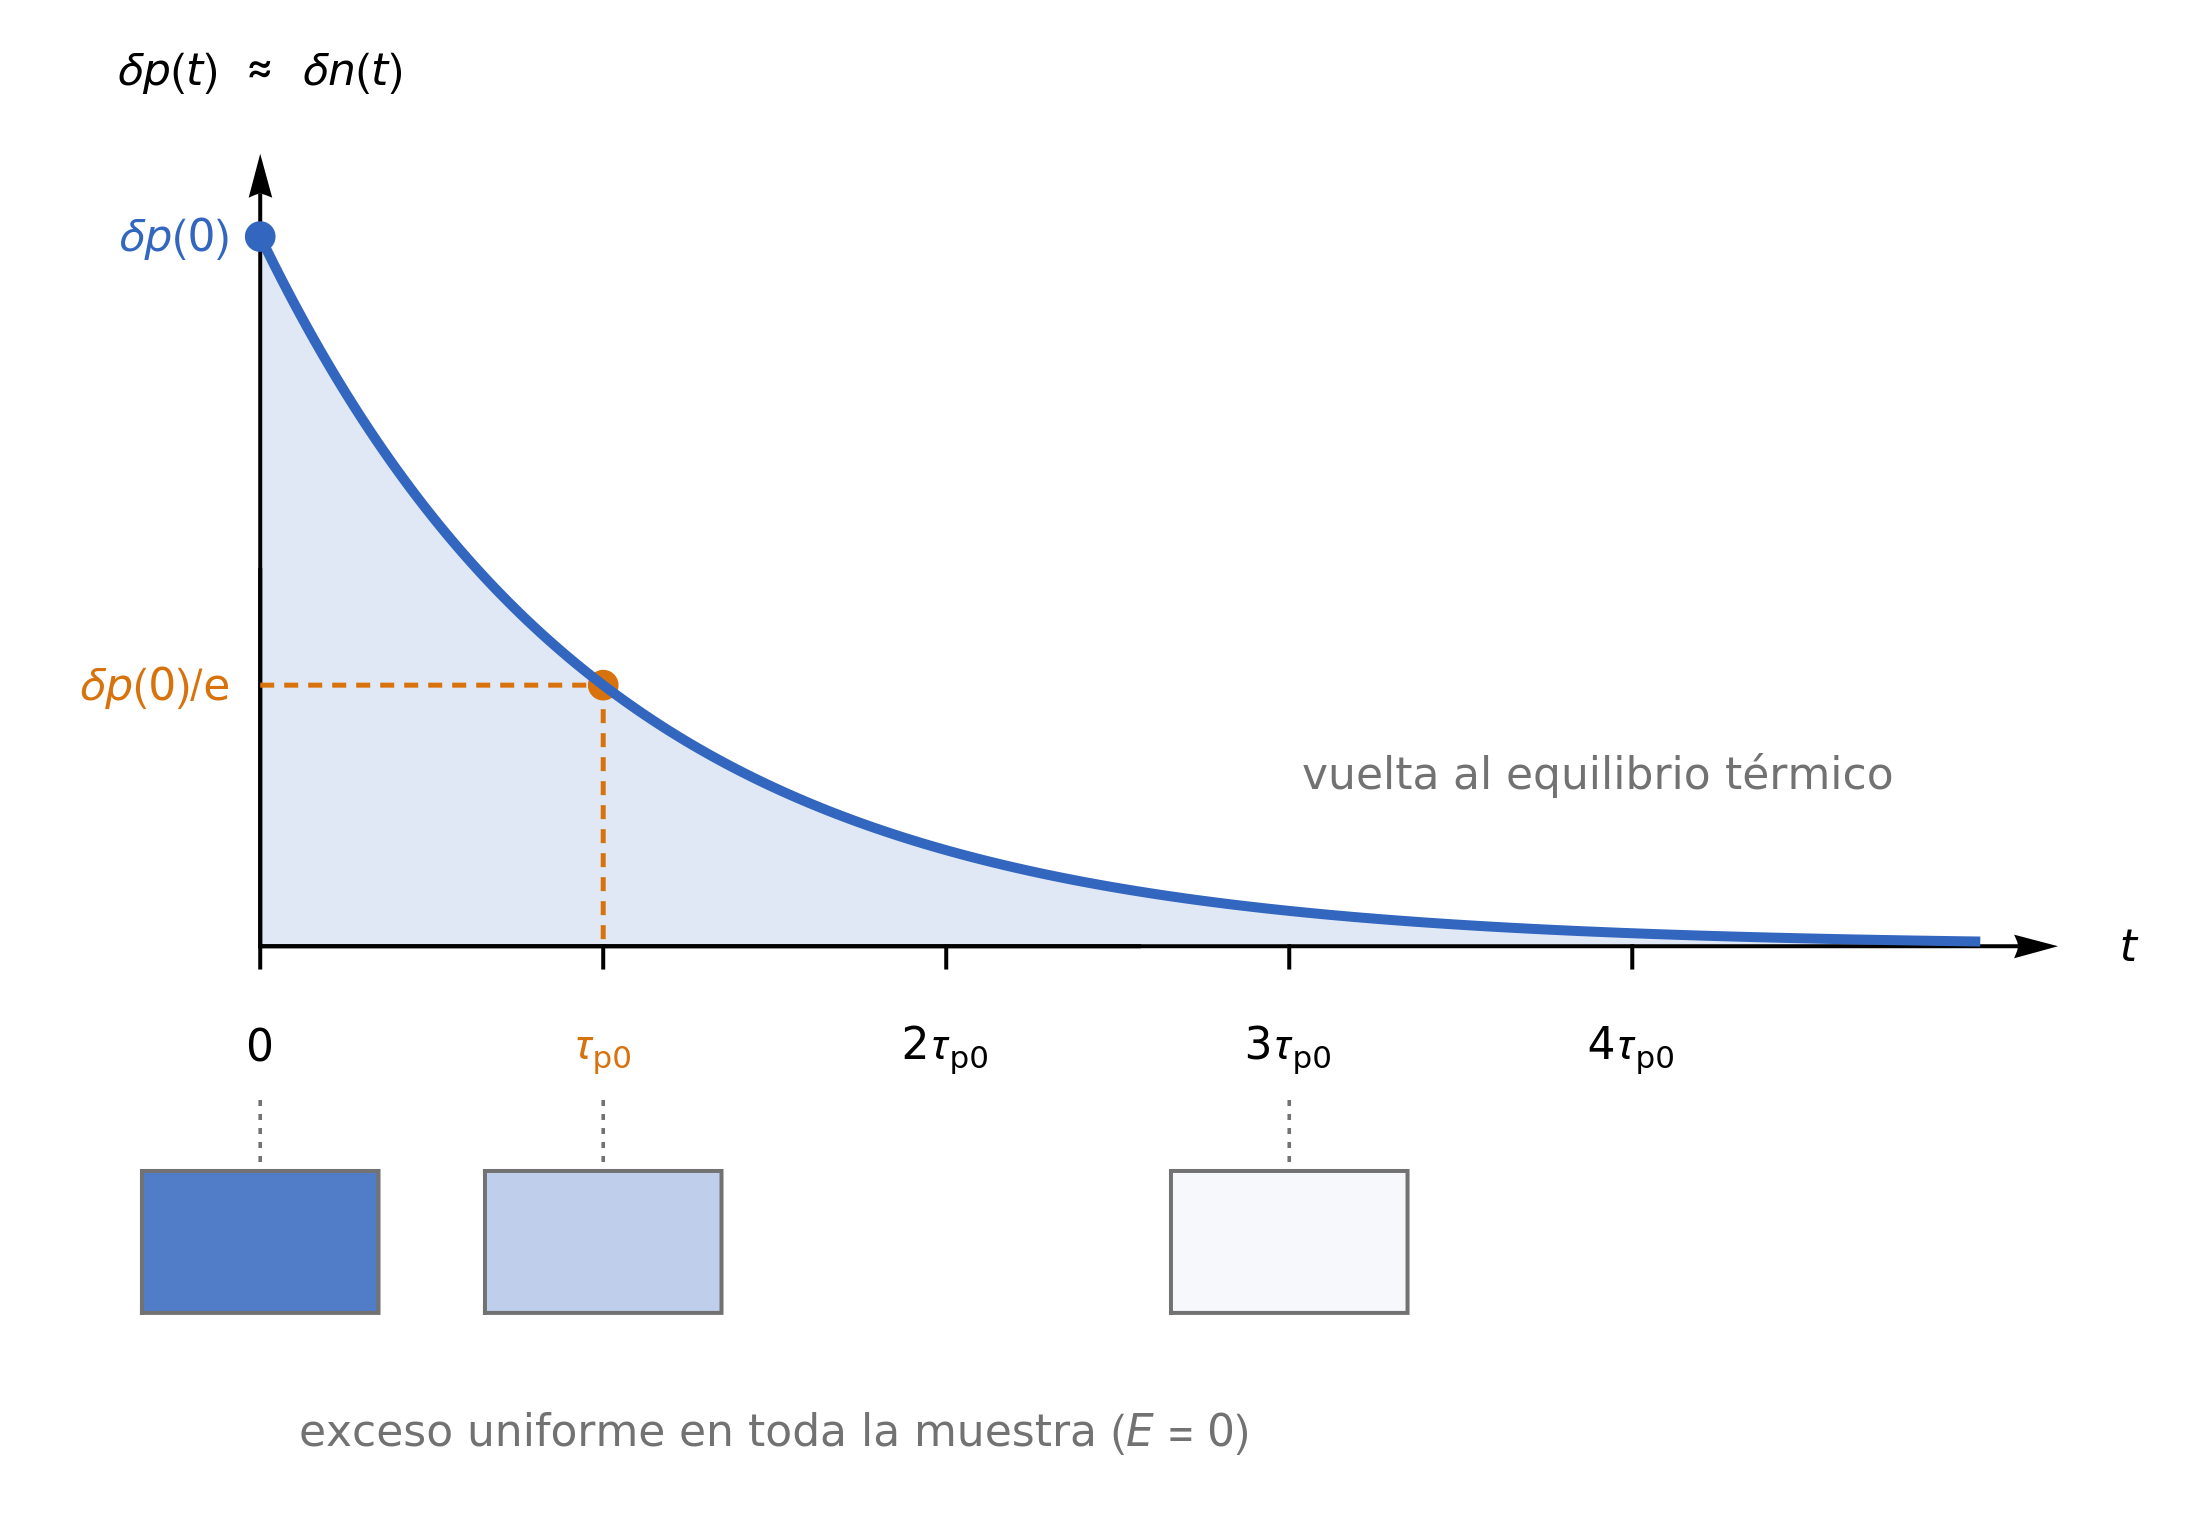
\includegraphics[width=0.55\linewidth]{imagenes/Tema3/T3_22.png}
\end{center}

\textbf{Interpretación física:} Tras el cese de la excitación externa, el exceso de portadores decae exponencialmente hasta anularse, devolviendo el semiconductor a sus concentraciones de equilibrio térmico ($n_0, p_0$). La constante de tiempo que gobierna esta relajación es la vida media de los portadores minoritarios ($\tau_{p0}$).
\end{ejemplo}

\begin{ejemplo}[Determinar la dependencia espacial estacionaria del exceso de concentración de portadores]
Considera un semiconductor tipo p homogéneo y de extensión infinita en una dimensión. Suponer campo eléctrico aplicado nulo ($E = 0$). El exceso de portadores es generado localmente en $x = 0$. Dichos portadores comenzarán a difundirse en las direcciones $x$ positiva y negativa. Calcular la distribución espacial del exceso de concentración de portadores $\delta n(x)$ en régimen estacionario.
\tcblower
Para un semiconductor tipo p, planteamos la ecuación de transporte ambipolar para la densidad de electrones minoritarios en exceso ($\delta n$):
\[
D_n \frac{\partial^2 (\delta n)}{\partial x^2} + \mu_n E \frac{\partial (\delta n)}{\partial x} + g' - \frac{\delta n}{\tau_{n0}} = \frac{\partial (\delta n)}{\partial t}
\]

De acuerdo con las hipótesis del problema:
\begin{enumerate}
    \item \textbf{Campo eléctrico nulo:} $E = 0$.
    \item \textbf{Sin generación continua fuera del origen:} $g' = 0$ para todo $x \neq 0$.
    \item \textbf{Régimen estacionario:} Las concentraciones no varían con el tiempo ($\frac{\partial (\delta n)}{\partial t} = 0$).
\end{enumerate}

Utilizando derivadas totales al tratarse de un problema unidimensional dependiente únicamente de $x$, la ecuación se reduce a:
\[
D_n \frac{d^2 (\delta n)}{dx^2} - \frac{\delta n}{\tau_{n0}} = 0
\]

Dividiendo entre el coeficiente de difusión $D_n$:
\[
\frac{d^2 (\delta n)}{dx^2} - \frac{\delta n}{D_n \tau_{n0}} = 0 \implies \frac{d^2 (\delta n)}{dx^2} - \frac{\delta n}{L_n^2} = 0
\]
donde se ha definido la \textbf{longitud de difusión de electrones} como $L_n = \sqrt{D_n \tau_{n0}}$.

La solución general de esta ecuación diferencial ordinaria homogénea de segundo orden se plantea por regiones:
\begin{itemize}
    \item \textbf{Región $x > 0$:} $\delta n(x) = A_1 e^{-x/L_n} + B_1 e^{x/L_n}$
    \item \textbf{Región $x < 0$:} $\delta n(x) = A_2 e^{x/L_n} + B_2 e^{-x/L_n}$
\end{itemize}

Aplicamos las \textbf{condiciones de contorno físicas}:
\begin{enumerate}
    \item Al alejarnos indefinidamente de la fuente de generación ($x \to \pm \infty$), el exceso de portadores debe ser finito y tender a cero:
    \[
    \lim_{x \to +\infty} \delta n(x) = 0 \implies B_1 = 0
    \]
    \[
    \lim_{x \to -\infty} \delta n(x) = 0 \implies B_2 = 0
    \]
    \item En el plano de generación $x = 0$, por continuidad del perfil de densidad y simetría del medio:
    \[
    \delta n(0^+) = \delta n(0^-) = \delta n(0) \implies A_1 = A_2 = \delta n(0)
    \]
\end{enumerate}

Unificando ambas regiones mediante la función valor absoluto, obtenemos el perfil espacial del exceso de portadores:
\[
\delta n(x) = \delta n(0) \exp\left( -\frac{|x|}{L_n} \right)
\]

Por la condición de cuasi-neutralidad eléctrica ($\delta p(x) \approx \delta n(x)$), el exceso de huecos mayoritarios presenta exactamente la misma distribución perfilada.

\begin{center}
    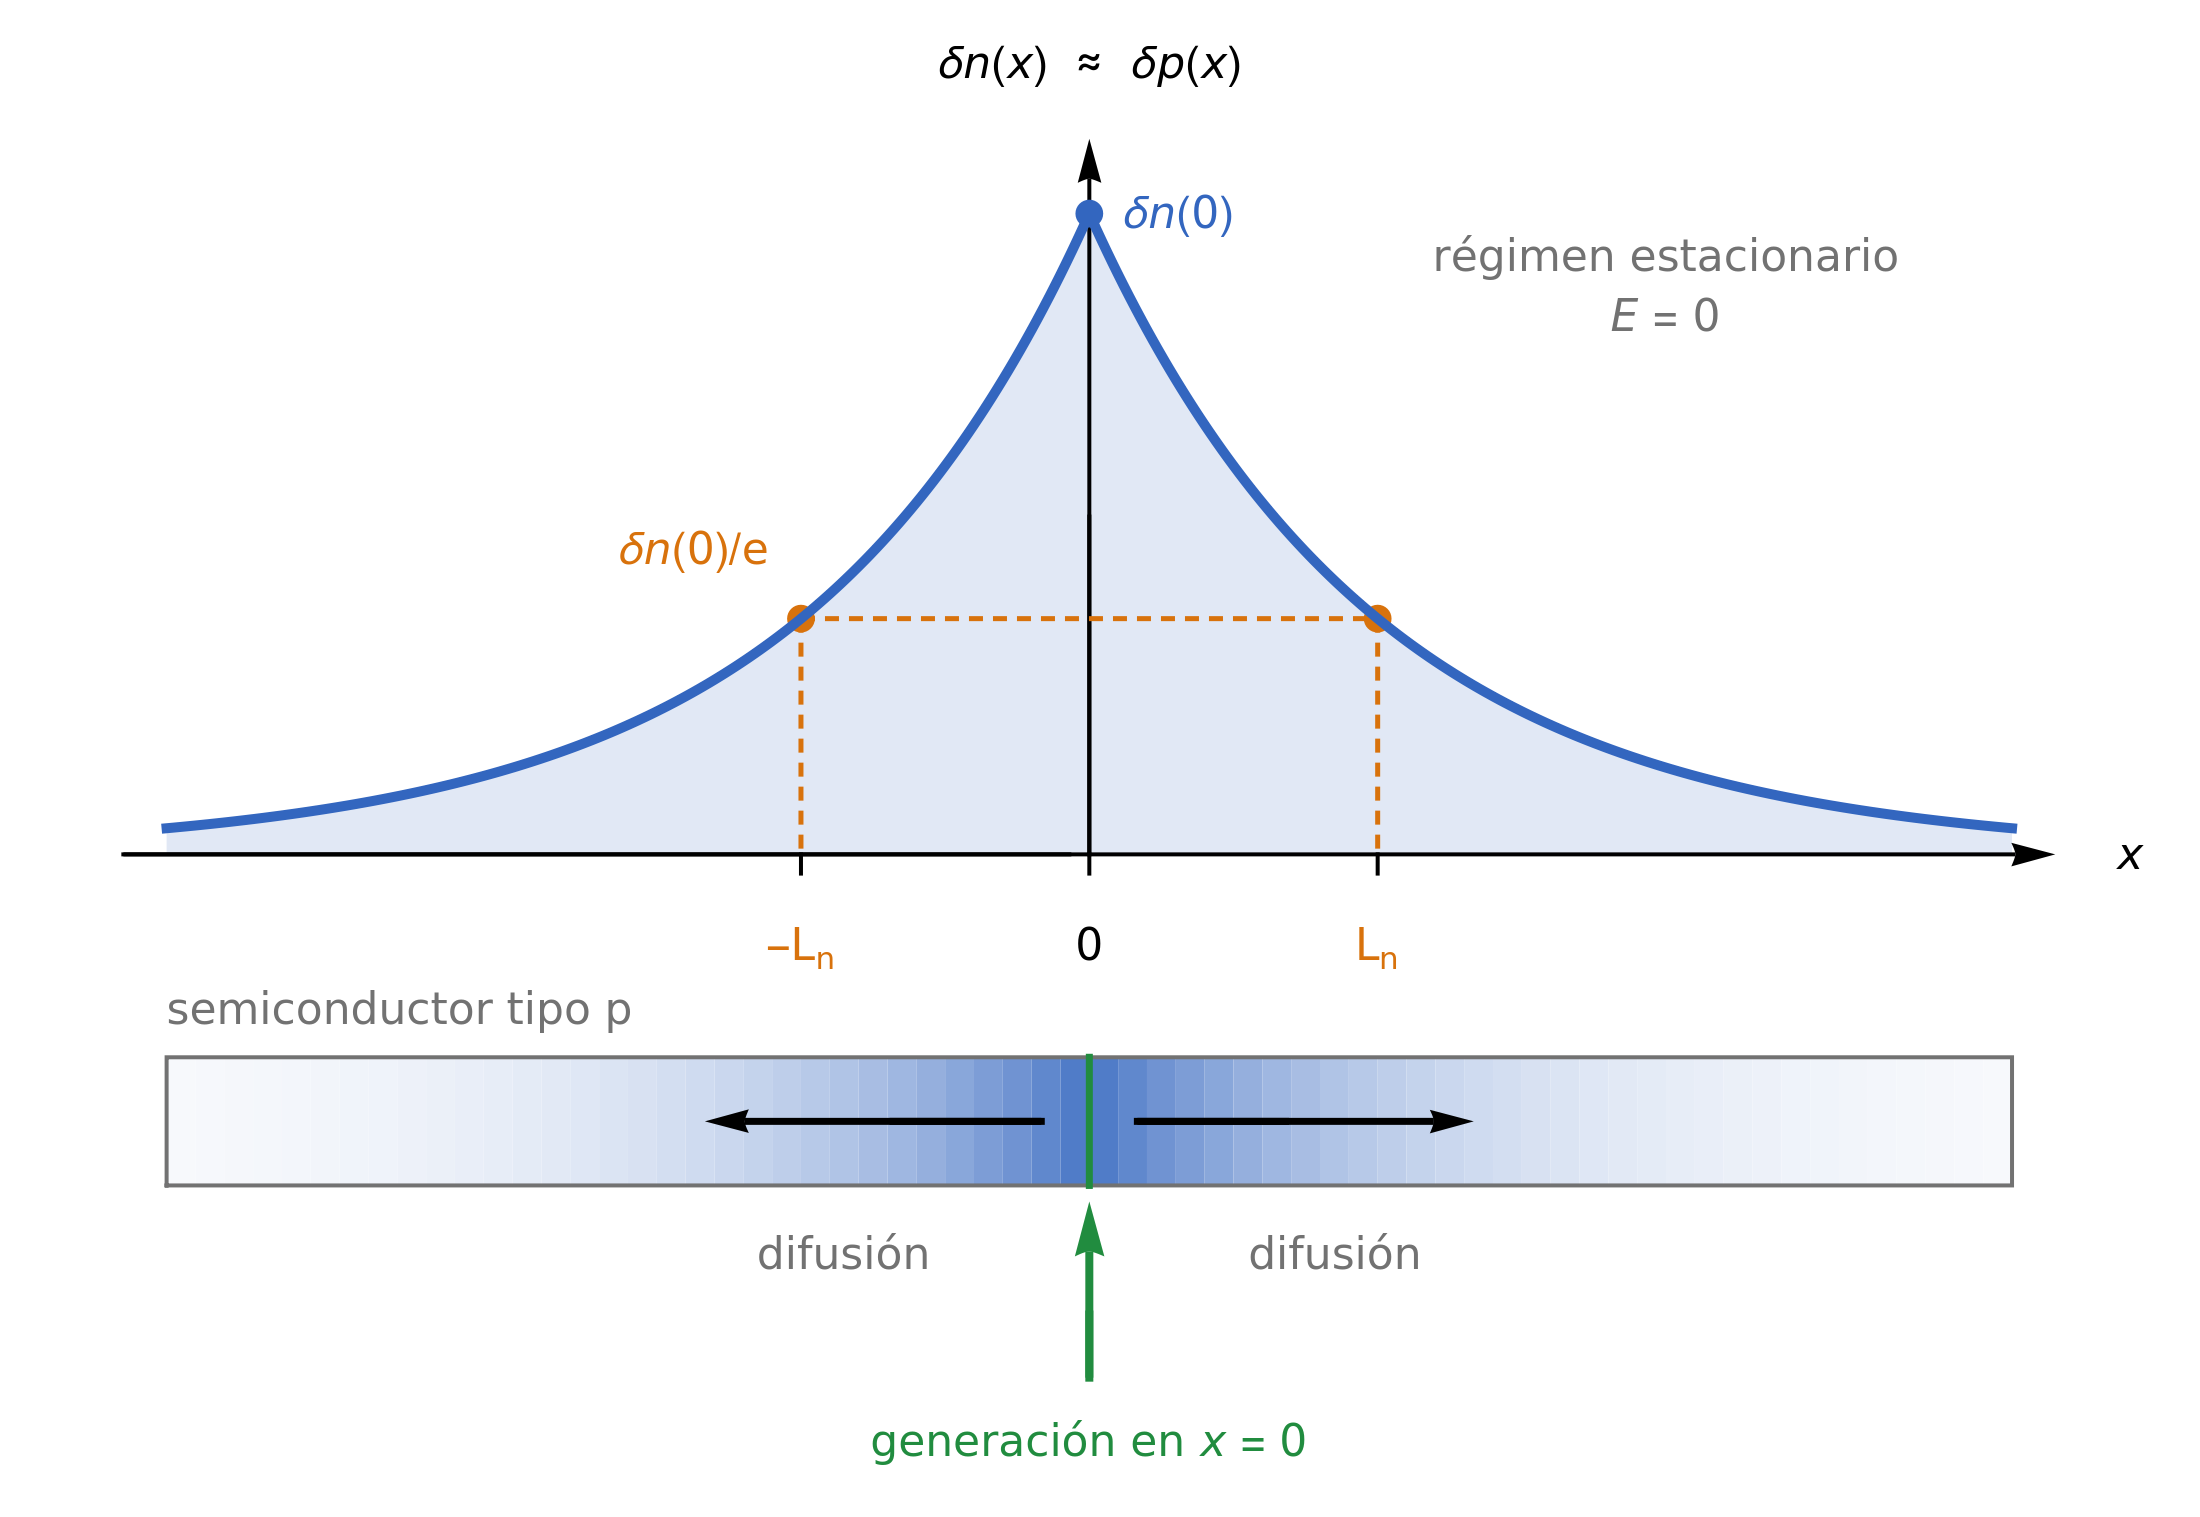
\includegraphics[width=0.55\linewidth]{imagenes/Tema3/T3_23.png}
\end{center}

\textbf{Interpretación física:} La concentración de portadores en exceso alcanza su valor máximo $\delta n(0)$ en el plano de generación y disminuye exponencialmente a medida que los portadores se difunden hacia las regiones adyacentes mientras se recombinan. La longitud de difusión $L_n$ representa la distancia media que se desplaza un portador minoritario por difusión antes de recombinarse con un portador mayoritario.
\end{ejemplo}